\chapter{Resultados e Discussões} \label{cap:resultados}

Neste capítulo, são apresentados os resultados obtidos pela execução da metodologia proposta no \autoref{cap:desenvolvimento}, acompanhados de discussões sobre os mesmos. A análise dos resultados é realizada com base nos cenários de ataques cibernéticos descritos na \autoref{sec:attacks}, com o objetivo de avaliar a robustez das redes industriais OPC UA e a variação no desempenho dos componentes quando submetidos a esses cenários. Para melhor organização das informações, os resultados são divididos em seções correspondentes a cada etapa da metodologia apresentada.

De modo geral, espera-se fornecer informações valiosas sobre as vulnerabilidades potenciais que podem ser expostas durante o processo de experimentação. Caso essas prospecções sejam confirmadas, elas podem contribuir para avanços futuros no protocolo OPC UA e nos sistemas IACS, fortalecendo ainda mais a robustez e a resistência destes contra ameaças cibernéticas em constante evolução.

\section{Implementação da Bancada Experimental} \label{sec:impl-bancada}

    A \autoref{fig:banc} apresenta a bancada experimental utilizada para ensaios de segurança cibernética, composta por um servidor OPC UA, um cliente OPC UA e um \textit{firewall} industrial. O servidor OPC UA é responsável por disponibilizar os dados de processo e controlar o sistema de automação industrial, enquanto o cliente OPC UA acessa e visualiza esses dados. O \textit{firewall} industrial é utilizado para monitorar e controlar o tráfego de dados entre o servidor e o cliente, assegurando a segurança da rede.

    \begin{figure}[htbp!]
        \caption{\label{fig:banc}Bancada experimental para ensaios de segurança cibernética}
        \begin{center}
            \includegraphics[width=0.5\textwidth]{USPSC-img/cyberkit2.png}
        \end{center}
        \legend{Fonte: elaborada pelo autor.}
    \end{figure}

\section{Aquisição dos Dados nos Cenários de Ataques Cibernéticos} \label{sec:exec-attacks}

    No passo da metodologia apresentado na \autoref{sec:aquisicao}, a bancada é colocada em operação de acordo com os cenários especificados (\autoref{tab:attacks}), aciona-se o sistema de medição, no qual são realizados a aquisição do tráfego da rede e o monitoramento do desempenho do hospedeiro do servidor OPC UA, e executam-se os respectivos ataques. Os dados de tráfego da rede OPC UA são coletados por 60 segundos para cada cenário.

    A \autoref{tab:carac-cenarios} apresenta um resumo detalhado das características do tráfego da rede e do desempenho em cada cenário de ataque e durante a comunicação normal em redes OPC UA industriais.

    \begin{table}[htbp!]
        \centering
        \caption{Informações do tráfego da rede e desempenho do hospedeiro em cada cenário}%
        \label{tab:carac-cenarios}
        \begin{tabular}{M{1.5cm}M{3cm}M{2.5cm}M{2.5cm}M{2cm}M{2cm}}
            \toprule
            \textbf{Cenário} & \textbf{\textit{Throughput} médio (kbits/s)} & \textbf{TP\textsuperscript{1} médio (Bytes)} & \textbf{PPS\textsuperscript{2} médio (pacotes/s)} & \textbf{Tráfego OPC UA (\%)} & \textbf{CPU\textsuperscript{3} (\%)} \\
            \toprule
            C1 & 130 & 127 & 128.4 & 28.7 & 7.31 \\
            \midrule
            C2 & 175 & 153 & 142.9 & 34.4 & 8.91 \\
            \midrule
            C3 & 179 & 162 & 138.3 & 31.8 & 9.01 \\
            \midrule
            C4 & 1166 & 965 & 151.1 & 9.2 & 17.16 \\
            \midrule
            C5 & 6824 & 972 & 877.9 & 5.3 & 10.64 \\
            \midrule
            C6 & 6894 & 973 & 885.9 & 8.2 & 10.78 \\
            \midrule
            C7 & 18000 & 60 & 38438.9 & 0.1 & 14.68 \\
            \midrule
            C8 & 12000 & 60 & 26788.9 & 0.1 & 13.23 \\
            \midrule
            C9 & 15000 & 60 & 31278.5 & 0.1 & 14.81 \\
            \midrule
            C10 & 462 & 171 & 337.3 & 72.9 & 9.86 \\
            \midrule
            C11 & 501 & 180 & 348.0 & 71.9 & 11.27 \\
            \midrule
            C12 & 491 & 184 & 334.1 & 69.8 & 11.36 \\
            \midrule
            C13 & 196 & 173 & 141.4 & 33.0 & 7.52 \\
            \midrule
            C14 & 235 & 195 & 151.3 & 35.2 & 9.03 \\
            \midrule
            C15 & 247 & 203 & 152.6 & 32.3 & 9.09 \\
            \midrule
            C16 & 105 & 125 & 105.3 & 33.1 & 6.80 \\
            \midrule
            C17 & 146 & 148 & 123.4 & 33.1 & 7.84 \\
            \midrule
            C18 & 137 & 159 & 107.9 & 33.2 & 7.96 \\
            \midrule
            C19 & 3410 & 43 & 10012.0 & 0.2 & 7.36 \\
            \midrule
            C20 & 3433 & 43 & 9896.4 & 0.2 & 7.97 \\
            \midrule
            C21 & 3432 & 44 & 9854.8 & 0.2 & 7.97 \\
            \midrule
            C22 & 168 & 127 & 166.1 & 32.1 & N/A \\
            \midrule
            C23 & 223 & 154 & 182.4 & 34.5 & N/A \\
            \midrule
            C24 & 219 & 162 & 169.7 & 32.5 & N/A \\
            \midrule
            C25 & 95 & 121 & 98.5 & 28.3 & 7.01 \\
            \midrule
            C26 & 253 & 142 & 222.7 & 17.9 & 7.95 \\
            \midrule
            C27 & 234 & 147 & 199.8 & 17.1 & 8.25 \\
            \bottomrule
            \multicolumn{6}{>{\tiny}l}{\textsuperscript{1} Tamanho do pacote.} \\
            \multicolumn{6}{>{\tiny}l}{\textsuperscript{2} Taxa de pacotes por segundo.} \\
            \multicolumn{6}{>{\tiny}l}{\textsuperscript{3} Processamento do hospedeiro do servidor OPC UA.} \\
        \end{tabular}
        \fonte{elaborada pelo autor.}%
    \end{table}

    O \textit{throughput} médio e a média do tamanho dos pacotes variam consideravelmente entre os cenários, indicando a intensidade do tráfego gerado em cada situação. Os diferentes cenários de ataques de DoS pelo loop infinito na cadeia de certificados, como C1, C2 e C3, apresentam uma taxa de transferência de dados relativamente baixa. Em contraste, cenários como C7, C8 e C9, que envolvem DoS pela inundação do TCP/IP, mostram um \textit{throughput} extremamente alto, refletindo a intensa carga imposta por esses ataques. Essa carga é evidenciada pelo indicador crítico da intensidade do tráfego, PPS (taxa de pacotes por segundo), que registra valores elevados nesses contextos.

    Já o percentual de tráfego OPC UA, apesar de variar drasticamente entre os cenários, não é considerado isoladamente um fator determinante para a severidade do ataque. Por exemplo, cenários com baixa porcentagem de tráfego OPC UA, como C7, C8 e C9, ainda podem gerar uma carga considerável na rede devido ao alto PPS. Por outro lado, cenários como C10, C11 e C12, que apresentam uma alta porcentagem de tráfego OPC UA, podem não necessariamente implicar em uma alta taxa de pacotes por segundo, mas indicam que o ataque está especificamente direcionado aos protocolos de comunicação OPC UA.

    Adicionalmente, o percentual de uso de processamento do controlador industrial (hospedeiro do servidor UA) é um indicador importante da carga imposta ao sistema durante os ataques. Cenários como C4, C5 e C6, que envolvem ataques de DoS pela chamada de vários métodos OPC UA nulos, mostram um aumento significativo no uso da CPU, indicando que esses ataques conseguem sobrecarregar o processamento do controlador, potencialmente levando à degradação do serviço ou à sua interrupção.

    Essa análise destaca a importância de considerar múltiplas métricas ao avaliar o impacto dos diferentes tipos de ataques na rede OPC UA. Além da taxa de transferência e de pacotes por segundo, o tamanho dos pacotes e o percentual de tráfego OPC UA são essenciais para uma compreensão abrangente do comportamento da rede sob diferentes condições de ataque. A análise detalhada dessas variáveis pode fornecer percepções valiosas para o desenvolvimento de estratégias de mitigação e a implementação de medidas de segurança mais eficazes em ambientes industriais.

\section{Processamento dos Dados} \label{sec:processamento-dados}

    Após a coleta dos dados de tráfego da rede e do desempenho do hospedeiro do servidor OPC UA para cada cenário de ataque, o passo seguinte é processar essas informações para posterior análise e interpretação. Esse processamento é realizado pelo aplicativo \textbf{uanalyser}, que tem a função de extrair dados relevantes dos valores brutos e gerar métricas de desempenho específicas para cada situação.

    Na versão atual do aplicativo (v1.0.0), são gerados gráficos de (a) \textit{Throughput} (kbps), (b) desempenho do hospedeiro do servidor OPC UA (RAM e CPU), (c) quantidade de pacotes OPC UA por segundo e (d) \textit{Round Trip Time} (RTT) normalizado por pacote. A figura \autoref{fig:0-normal-local-server} apresenta um exemplo dos quatro gráficos de saída do aplicativo para o cenário C25.

    \begin{figure}[htbp!]
        \centering
        \caption{\label{fig:0-normal-local-server}Gráficos de condição normal de operação - nível de segurança: `None'.}
        \begin{subfigure}[t]{0.5\textwidth}
            \centering
            \caption{\textit{Throughput}}
            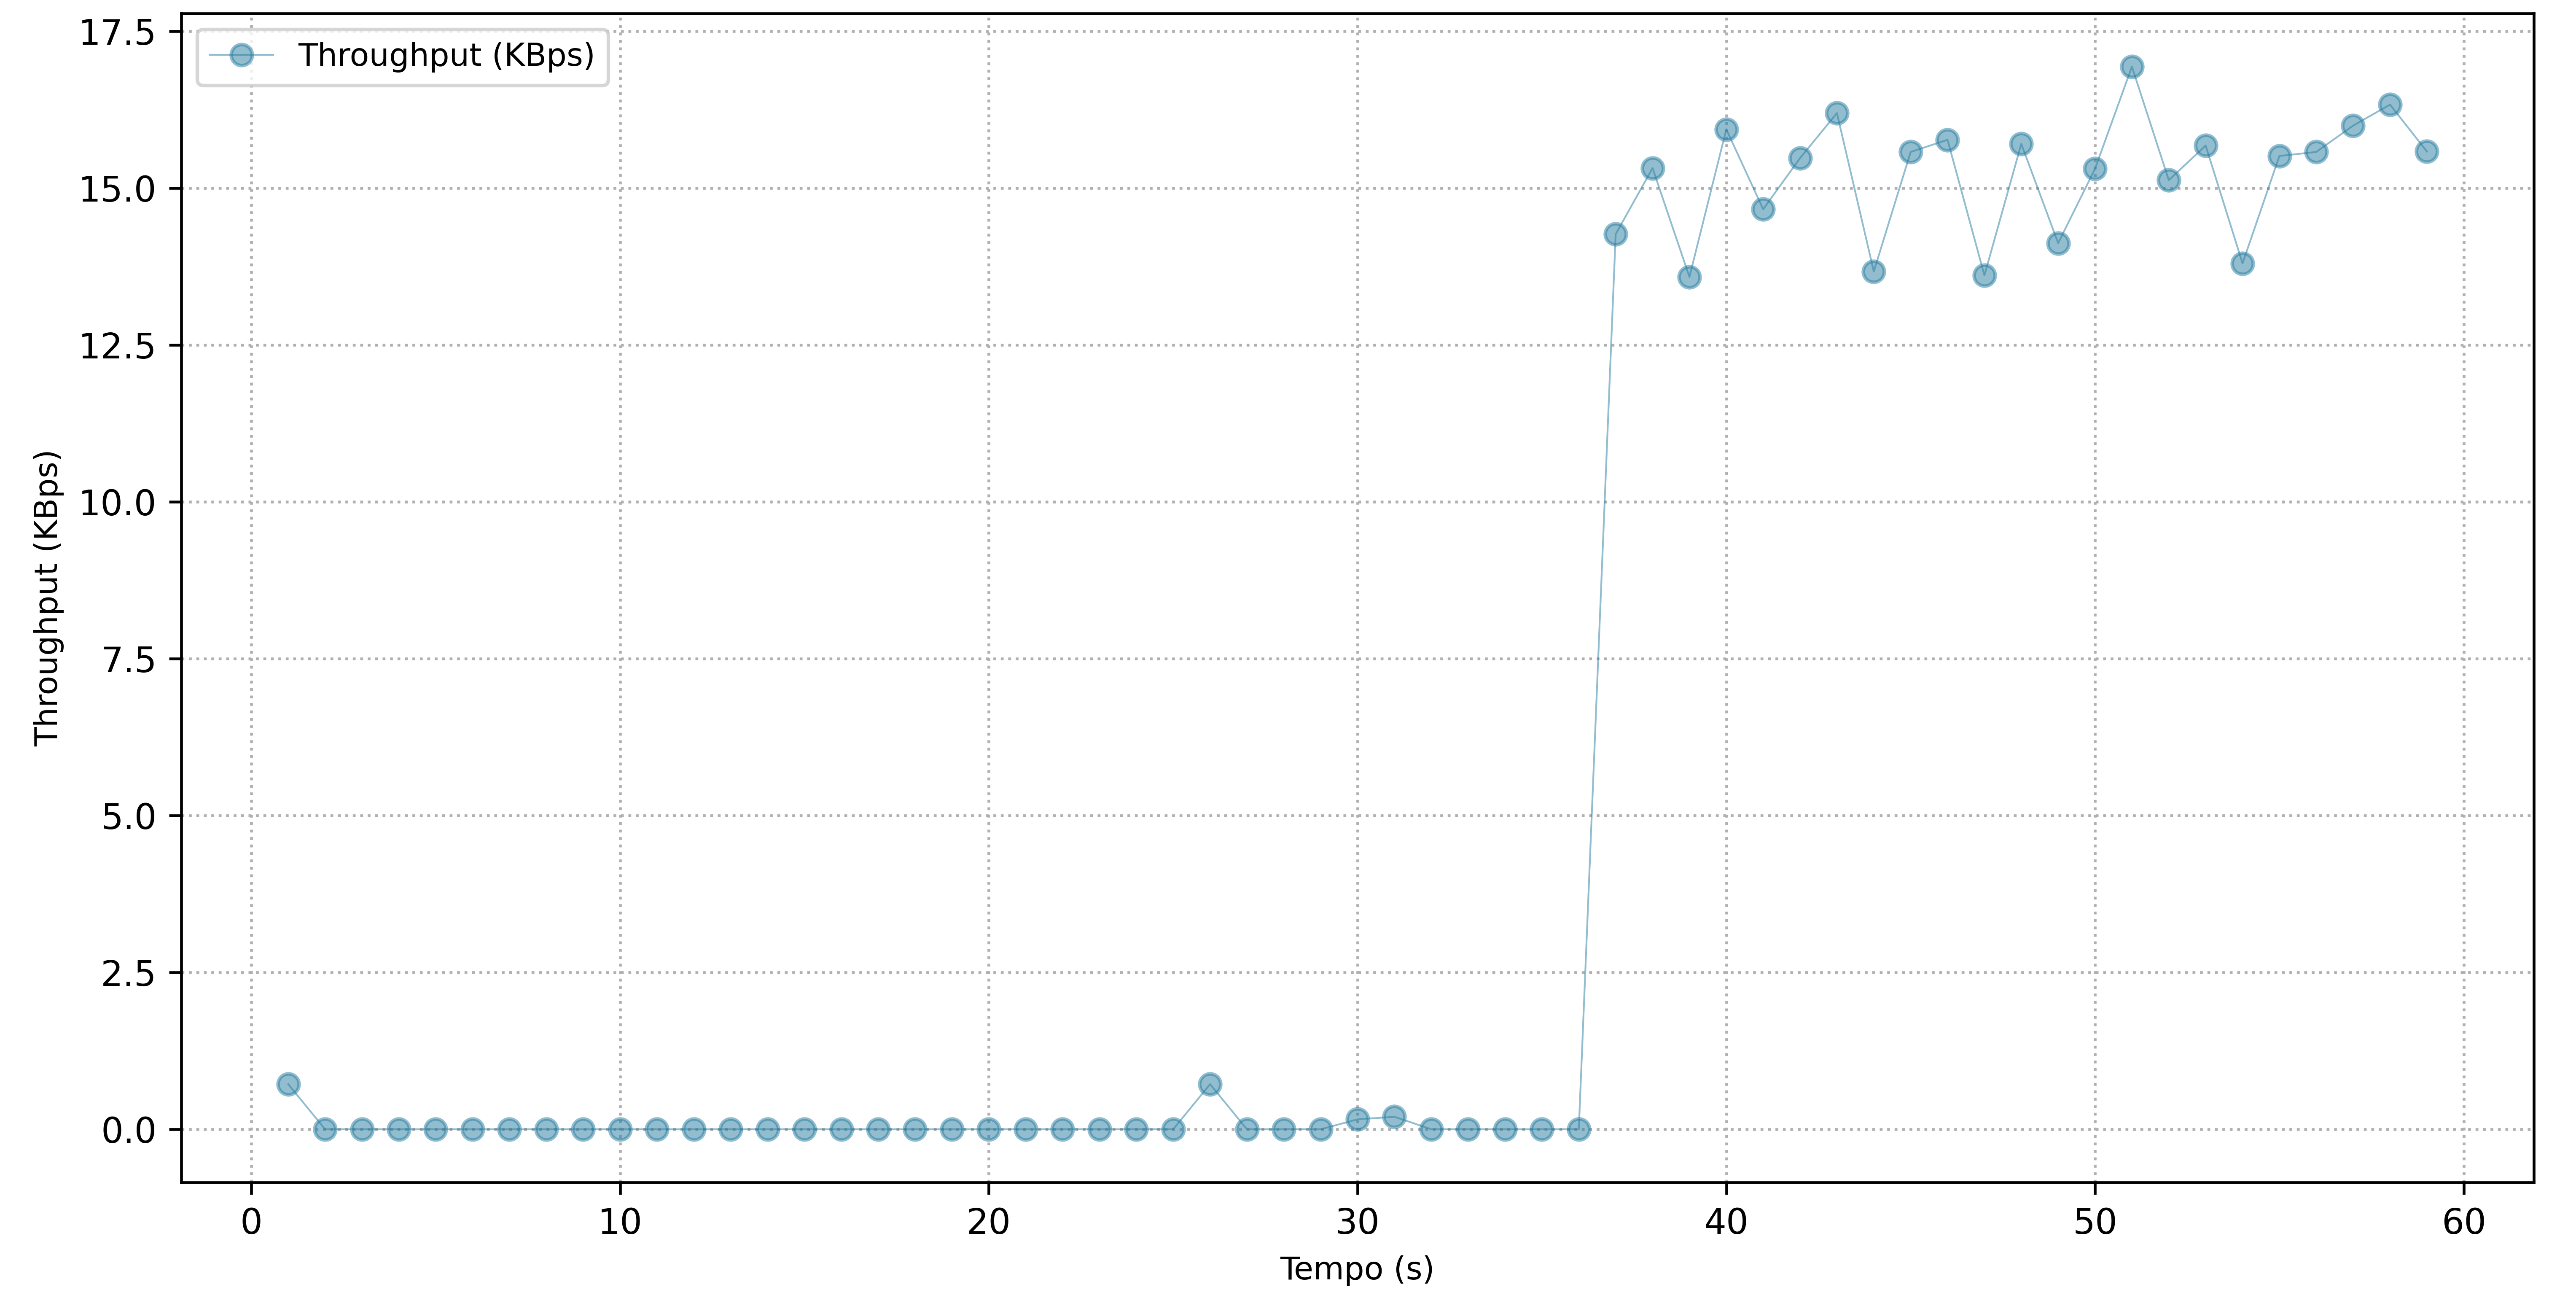
\includegraphics[width=1\textwidth, height=120pt]{USPSC-img/output/cropped/0-normal_local_server-tput.png}
        \end{subfigure}%
        ~ 
        \begin{subfigure}[t]{0.5\textwidth}
            \centering
            \caption{Desempenho}
            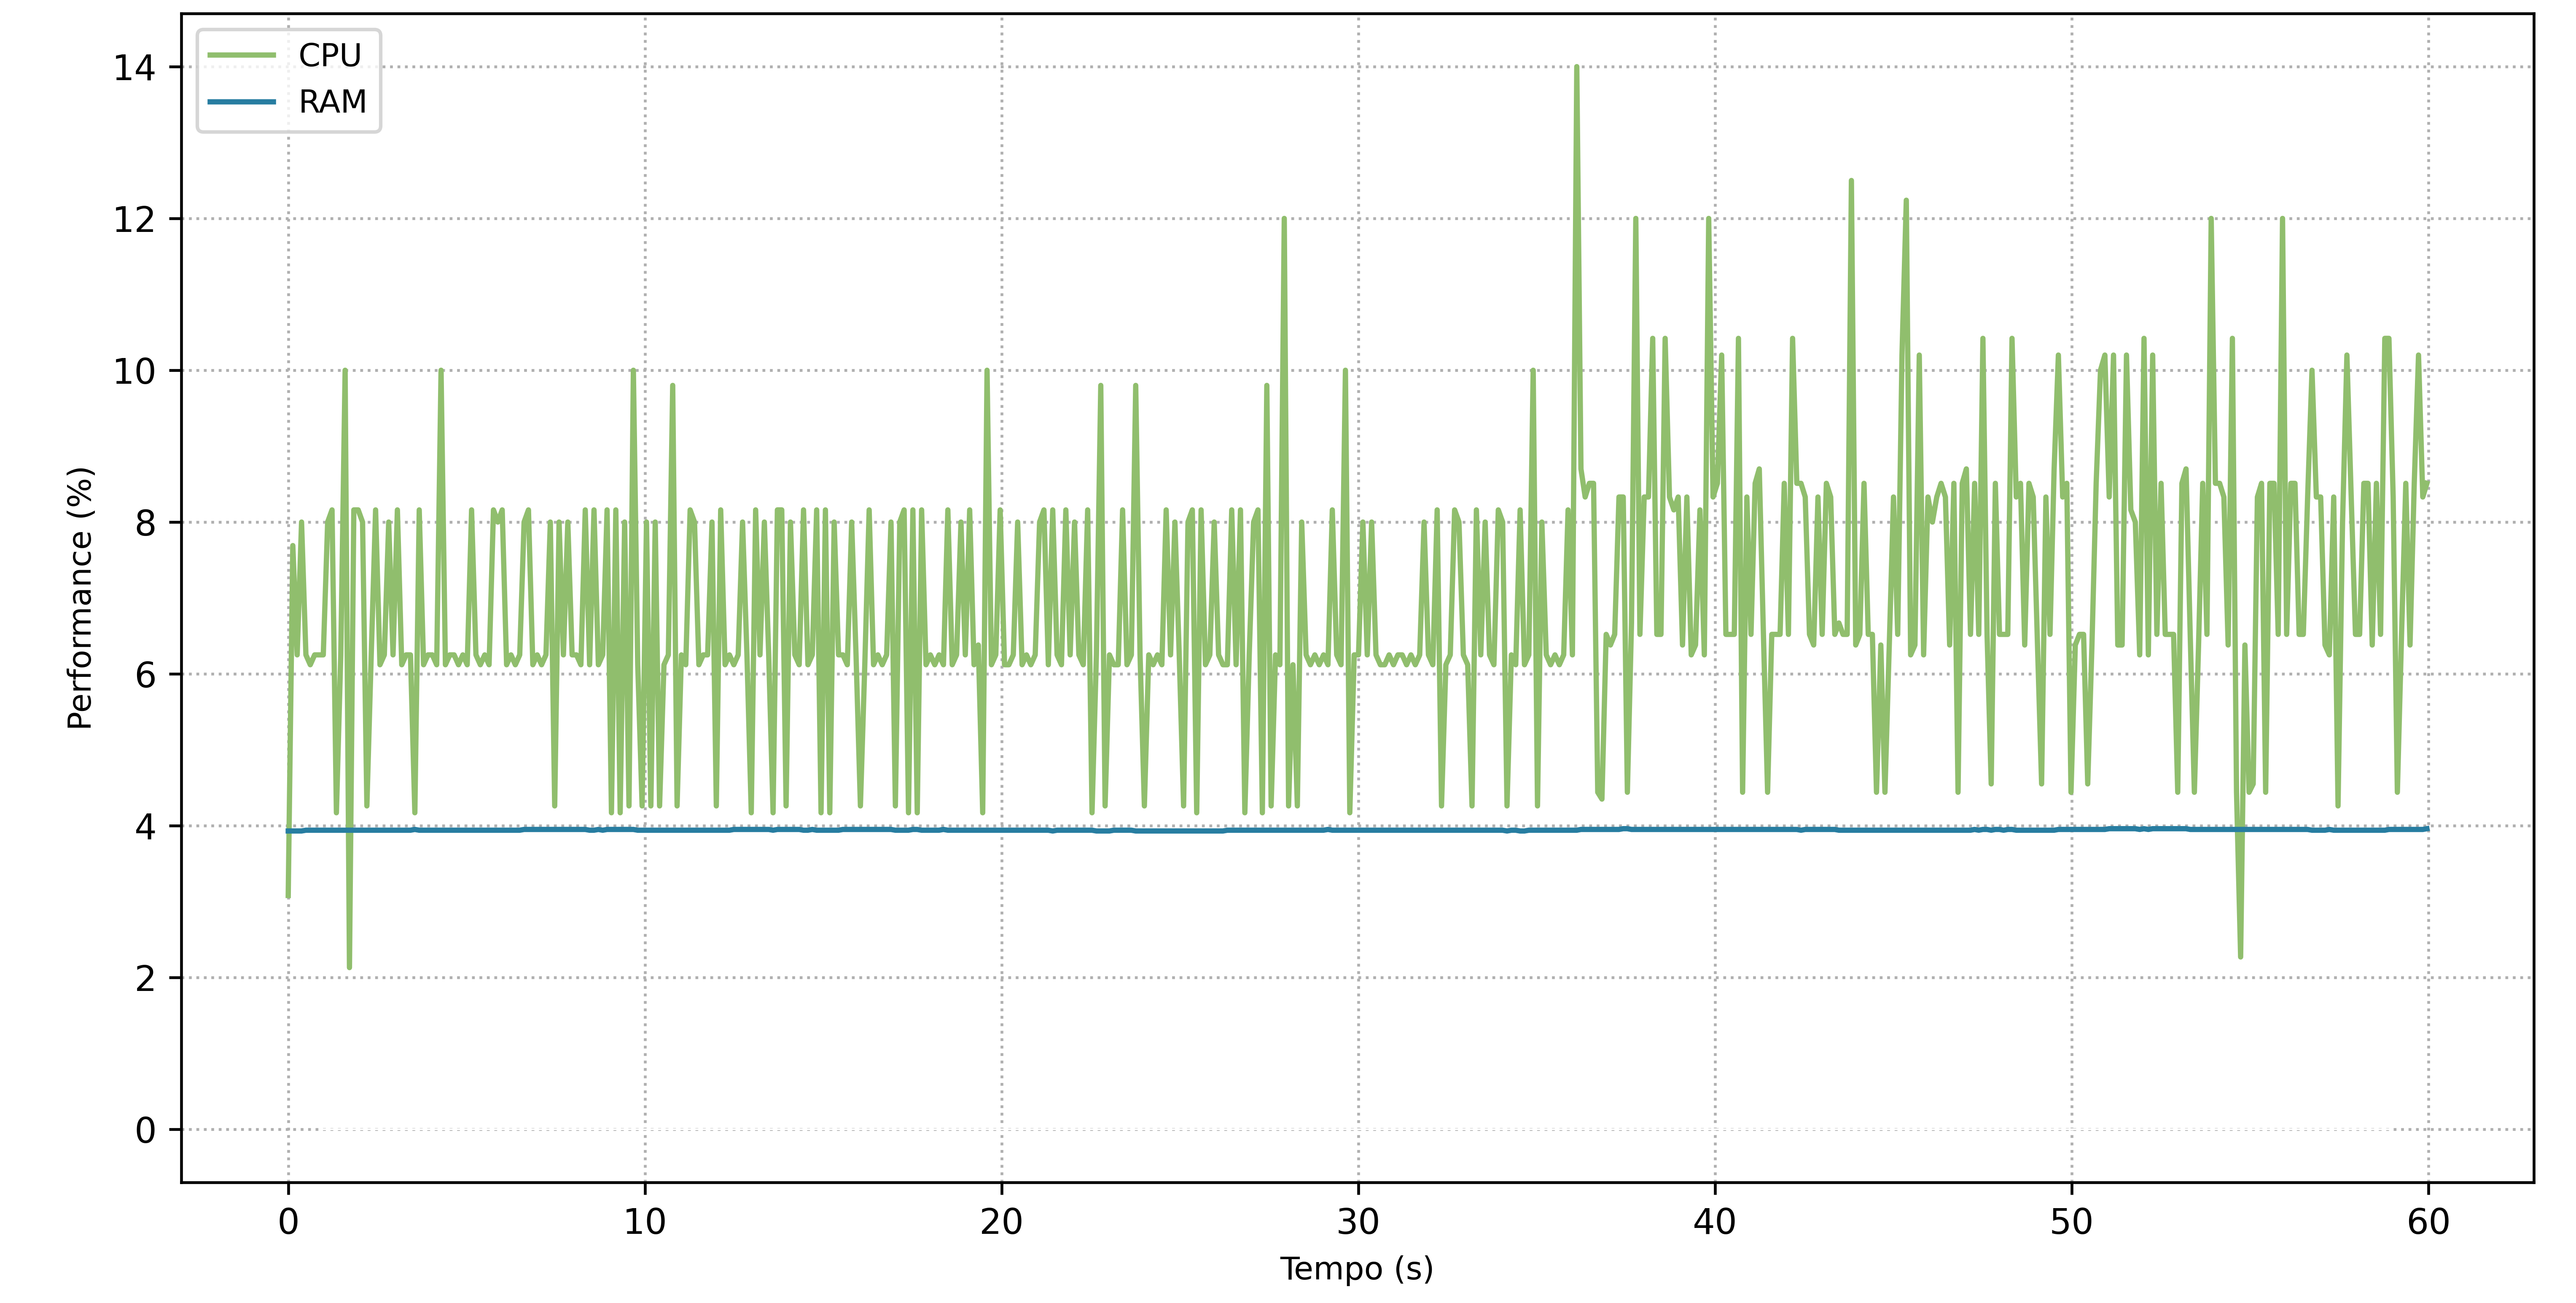
\includegraphics[width=1\textwidth, height=120pt]{USPSC-img/output/cropped/0-normal_local_server-perf.png}
        \end{subfigure}%
        \\
        \begin{subfigure}[t]{0.5\textwidth}
            \centering
            \caption{Pacotes OPC UA}
            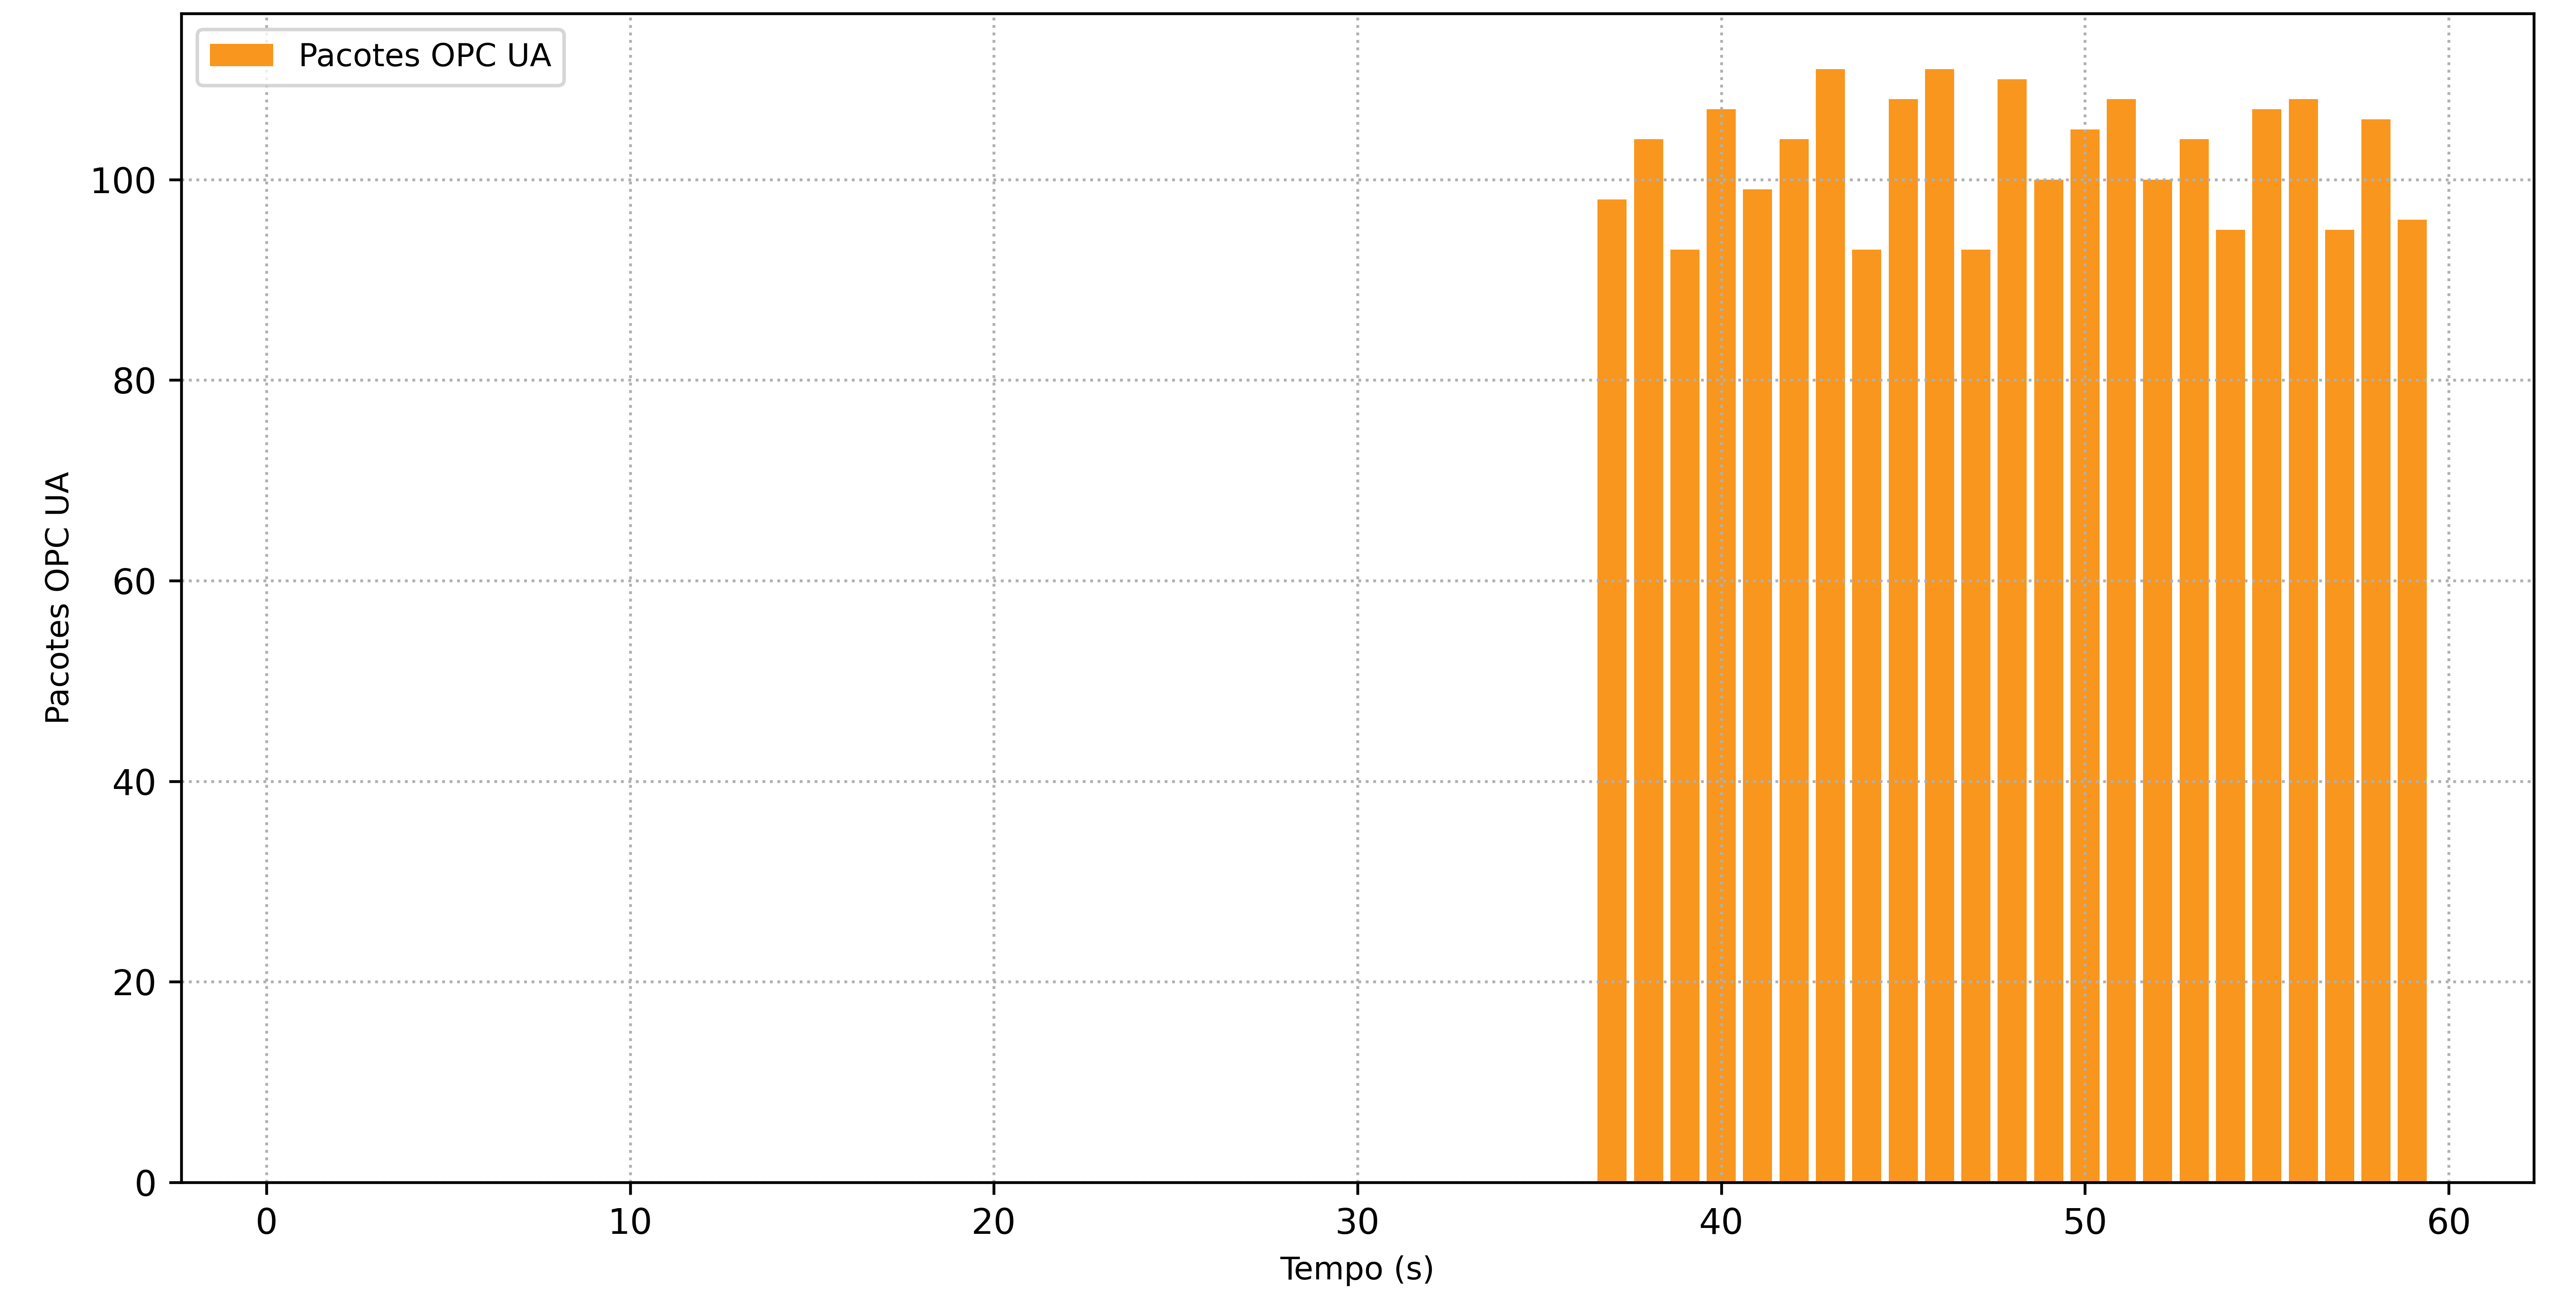
\includegraphics[width=1\textwidth, height=120pt]{USPSC-img/output/cropped/0-normal_local_server-pack.png}
        \end{subfigure}%
        ~
        \begin{subfigure}[t]{0.5\textwidth}
            \centering
            \caption{RTT por pacote}
            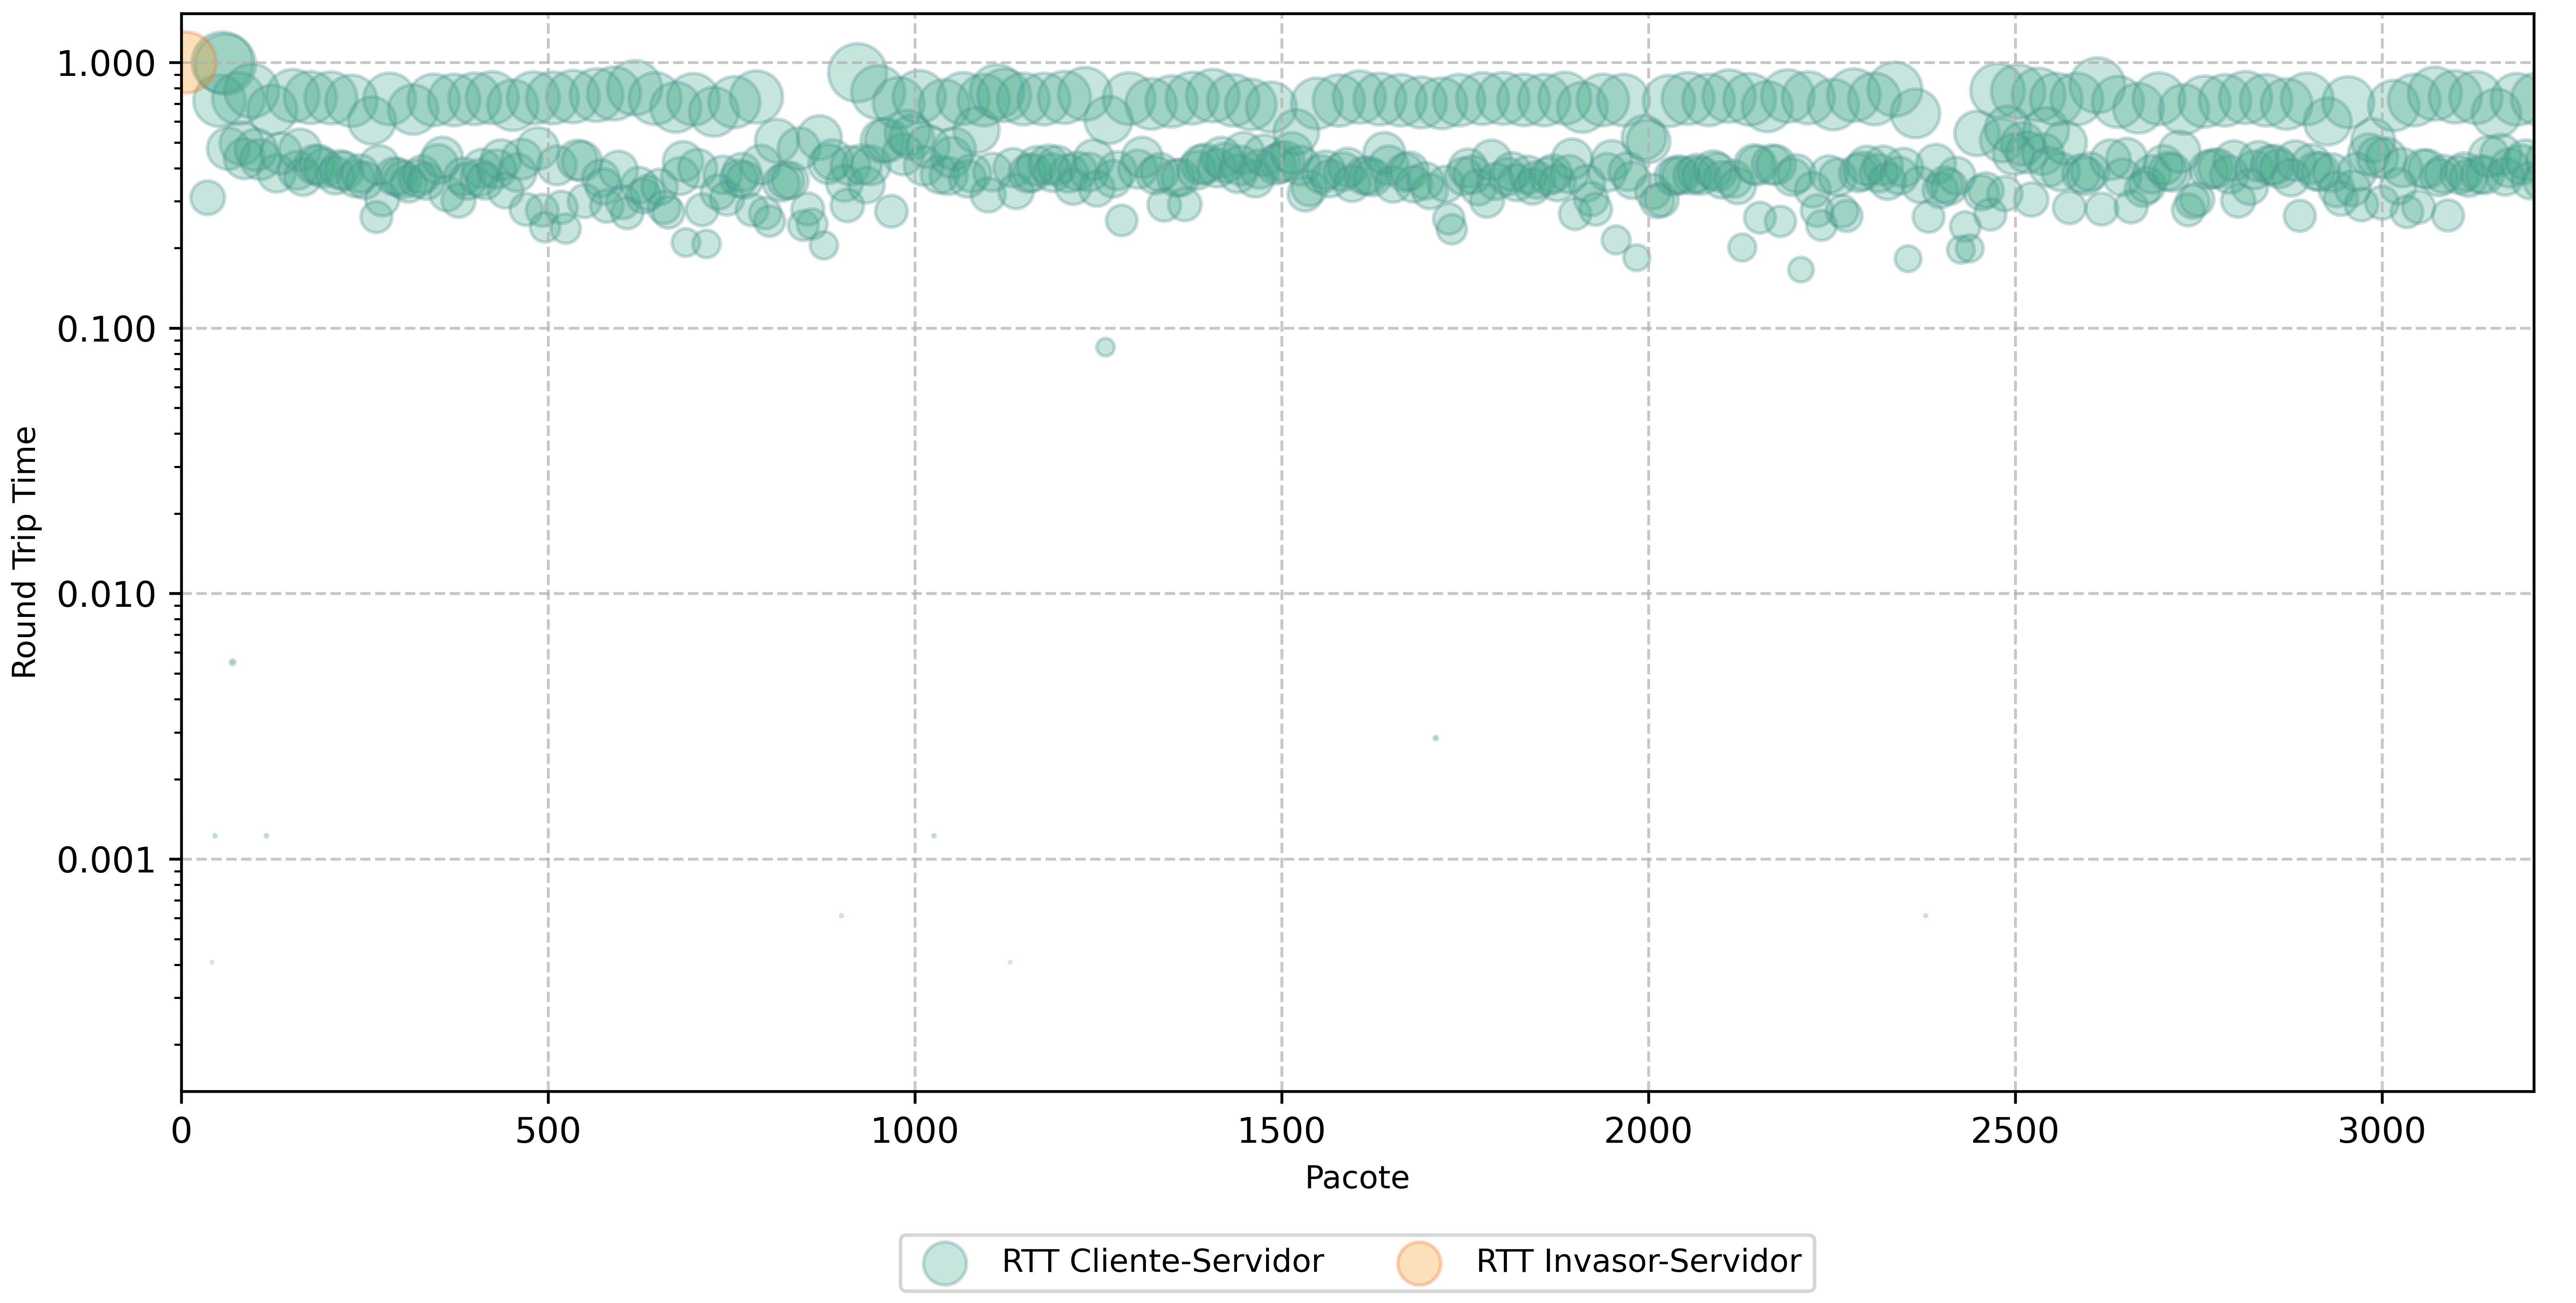
\includegraphics[width=1\textwidth, height=120pt]{USPSC-img/output/cropped/0-normal_local_server-rttp.png}
        \end{subfigure}%
        \legend{Fonte: elaborada pelo autor.}
    \end{figure}

    Os gráficos gerados para os demais cenários podem ser visualizados no \autoref{ap:graficos}.

\section{Análise dos Resultados} \label{sec:analise-resultados}

    Nesta seção, são apresentadas as análises dos resultados obtidos a partir dos cenários de ataques cibernéticos executados na bancada experimental. A análise é realizada com base nas métricas de desempenho obtidas dos dados coletados, com o objetivo de avaliar a robustez das redes industriais OPC UA e a variação no desempenho dos componentes ao serem submetidos a tais cenários. Para uma melhor organização das informações, os resultados são divididos em seções correspondentes a cada tipo de ataque.

    \subsection{\textit{Packet Sniffing}}

        Com o auxílio do Wireshark e do Ettercap, este primeiro ataque foi realizado com o objetivo de identificar a presença de vulnerabilidades na rede OPC UA que permitam a interceptação não autorizada de pacotes. Inicialmente, o Ettercap foi utilizado para a captura unificada de pacotes, enquanto o Wireshark se encarregou da análise detalhada do tráfego de rede. Uma vez que o servidor e o cliente estão conectados, estabelece-se um canal seguro para comunicação. No entanto, o atacante pode explorar vulnerabilidades na rede para interceptar pacotes e obter informações confidenciais, como os endereços IP e MAC de todos os dispositivos conectados. No início da captura para os cenários C22, C23 e C24, é possível observar a presença de pacotes de comunicação entre o servidor e o cliente, conforme ilustrado na \autoref{fig:0-sniffing-wireshark}. Note que foi aplicado um filtro para exibir apenas os pacotes de comunicação OPC UA, omitindo todos os outros dados nesta visualização. Todo o tráfego relevante relacionado ao protocolo OPC UA, apresentado na \autoref{fig:seqConn}, é analisado pelo Wireshark.

        \begin{figure}[htbp!]
            \caption{\label{fig:0-sniffing-wireshark}Comunicação interceptada entre o servidor e o cliente OPC UA com modo de segurança `None'}
            \begin{center}
                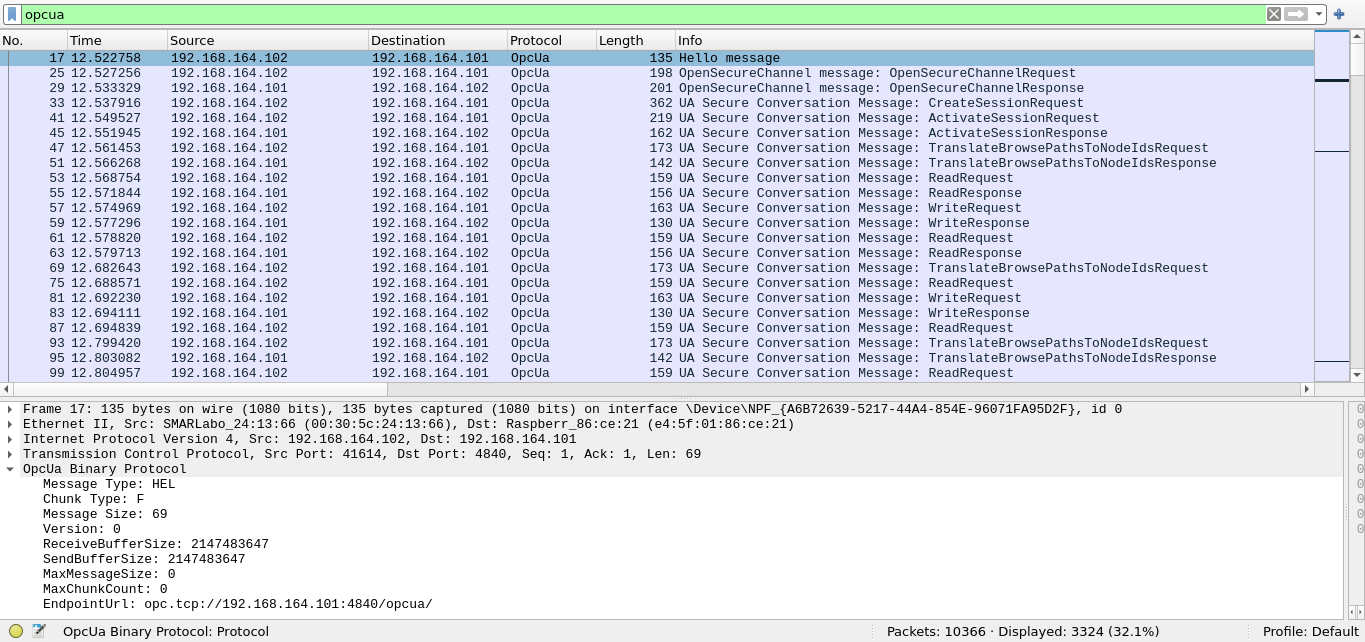
\includegraphics[width=0.972\textwidth]{USPSC-img/0-sniffing-wireshark-filtered-anon.png}
            \end{center}
            \legend{Fonte: elaborada pelo autor.}
        \end{figure}

        Vale ressaltar que o invasor possui o endereço IP 192.168.164.115 e está apenas conectado à rede, sem interação física com o servidor (192.168.164.101) ou cliente (192.168.164.102). Na configuração da comunicação com os modos de segurança `None' e `Sign', é possível observar que o invasor consegue obter todos os dados sensíveis da comunicação entre o servidor e o cliente, conforme indicado na \autoref{fig:writeRequest}, que representa a coleta do pacote de requisição de escrita (\textit{UA Secure Conversation Message: WriteRequest}) do mesmo valor e nó, do cliente para o servidor.

        \begin{figure}[htbp!]
            \centering
            \caption{\label{fig:writeRequest}Informações obtidas pelo invasor com modo de segurança `None' e `Sign'}
            \begin{subfigure}[t]{0.5\textwidth}
                \centering
                \caption{`None'}
                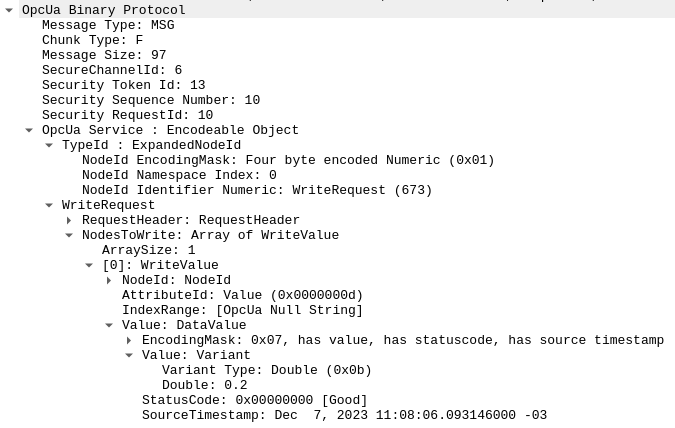
\includegraphics[width=1\textwidth]{USPSC-img/0-sniffing-WriteRequest.png}
            \end{subfigure}%
            ~ 
            \begin{subfigure}[t]{0.5\textwidth}
                \centering
                \caption{`Sign'}
                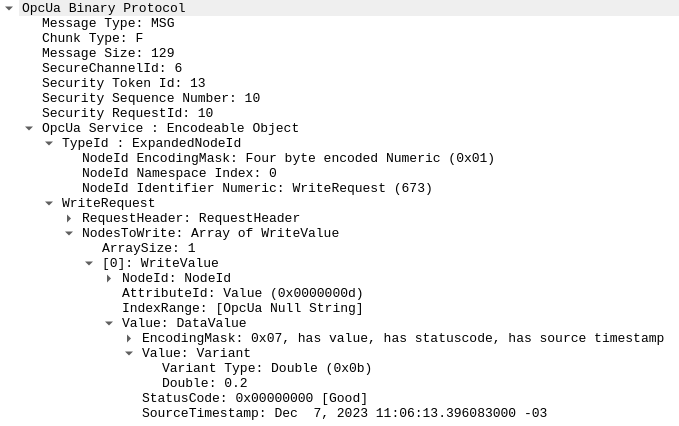
\includegraphics[width=1\textwidth]{USPSC-img/1-sniffing-WriteRequest.png}
            \end{subfigure}%
            \legend{Fonte: elaborada pelo autor.}
        \end{figure}

        No entanto, ao configurar a comunicação no modo de segurança `Sign \& Encrypt', o invasor não é capaz de obter informações sensíveis da comunicação entre o servidor e o cliente, pois os dados, além de assinados, são criptografados com políticas mais robustas, como a Basic256Sha256. Assim, no cenário C24, embora os dados da rede continuem sendo interceptados, a comunicação OPC UA não pode ser decifrada, uma vez que todos os pacotes do tipo MSG, com a informação \textit{UA Secure Conversation Message: ServiceId [ID]}, possuem o campo de dados \texttt{NodeId EncodingMask} desconhecido.

        Portanto, este ataque tem o potencial de comprometer a segurança da rede OPC UA ao quebrar a confidencialidade da comunicação, desde que esta seja configurada com modos de segurança mais fracos, como `None' e `Sign'. Tais cenários de ataque evidenciam que, utilizando ferramentas simples e tendo acesso ao componente principal da rede, um invasor pode facilmente realizar ataques de captura de pacotes na rede OPC UA, comprometendo dados confidenciais de toda a rede. O invasor é capaz de registrar todo o tráfego trocado e, posteriormente, utilizá-lo para outros tipos de ataques, como inserção de pacotes maliciosos (\textit{packet injection}), DoS, MITM, DDoS, entre outros.

    \subsection{\textit{Man in the Middle (MITM)}}

        Depois de realizar com sucesso o ataque de \textit{Packet Sniffing}, o invasor terá acesso a uma lista de endereços de todos os dispositivos da rede, além de obter informações sensíveis do hospedeiro do servidor OPC UA, incluindo o \texttt{EndpointURI}. Assim, o ataque MITM pode ser realizado, permitindo não apenas a interceptação dos dados, mas também o controle total da comunicação.

        Ambas as técnicas utilizadas para executar o ataque MITM foram realizadas com êxito. A execução por meio da falsificação da tabela ARP, nos cenários C16, C17 e C18, demonstra que a comunicação é interceptada e redirecionada para o invasor, possibilitando a captura e modificação dos pacotes de dados. A \autoref{fig:0-mitm-wireshark} demonstra a captura de pacotes de comunicação entre o servidor e o cliente, com o invasor atuando como intermediário. Ao comparar com o tráfego apresentado na \autoref{fig:0-sniffing-wireshark}, é possível observar que o fluxo normal de comunicação é interceptado e redirecionado para o invasor, identificado pelo endereço MAC \texttt{00:09:5B:A0:5F:F0}.

        \begin{figure}[htbp!]
            \centering
            \caption{\label{fig:0-mitm-wireshark}Interceptação de pacotes no ataque MITM com modo de segurança `None'}
            \begin{subfigure}[t]{1\textwidth}
                \centering
                \caption{\texttt{OpenSecureChannelRequest}}
                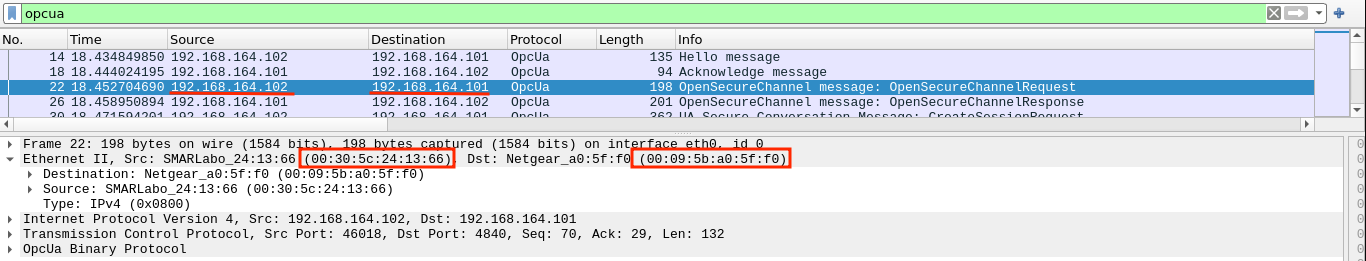
\includegraphics[width=1\textwidth]{USPSC-img/0-mitm-arp_1.png}
            \end{subfigure}%
            \\
            \begin{subfigure}[t]{1\textwidth}
                \centering
                \caption{\texttt{OpenSecureChannelResponse}}
                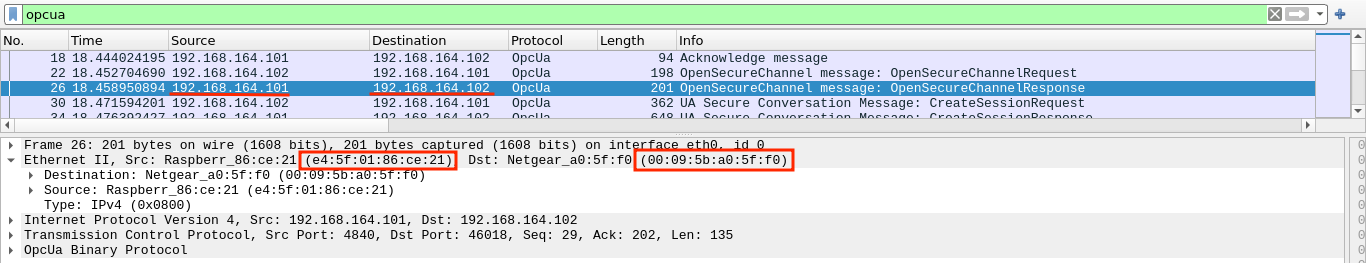
\includegraphics[width=1\textwidth]{USPSC-img/0-mitm-arp_2.png}
            \end{subfigure}%
            \legend{Fonte: elaborada pelo autor.}
        \end{figure}

        O processo começa com a etapa de handshake entre os agentes, onde o cliente inicia a comunicação, seguida pelo reconhecimento do servidor. Em seguida, o cliente envia uma solicitação \textit{OpenSecureChannelRequest}, à qual o servidor responde com uma \textit{OpenSecureChannelResponse}. Após essa etapa, é criado um \textit{SecureChannel}, e o cliente envia uma \textit{CreateSessionRequest}, que é respondida pelo servidor com uma \textit{CreateSessionResponse}. Uma vez que a sessão é criada, cliente e servidor se ativam usando \textit{ActivateSessionRequest} e \textit{ActivateSessionResponse}. A partir desse ponto, quando o cliente tenta acessar qualquer informação do servidor, observam-se as mensagens \textit{ReadRequest} e \textit{ReadResponse}.

        No ataque MITM pelo roubo de portas, nos cenários C19, C20 e C21, observa-se um aumento significativo no \texttt{throughput}, alcançando valores dez vezes maiores que os registrados na falsificação da tabela ARP. Essa elevação ocorre devido ao processo de roubo de portas, no qual a rede é inundada com pacotes ARP para saturar a tabela ARP do servidor, forçando-o a redirecionar o tráfego para o invasor. Em média, 99,3\% dos pacotes nesses cenários são provenientes do \textit{broadcast} ARP. No entanto, mesmo quando essa técnica é empregada com sucesso e a interceptação é efetuada, nota-se que a comunicação não ocorre diretamente através do invasor, mas sim entre o servidor e o cliente, com o redirecionamento dessa comunicação para a porta roubada pelo invasor.
        
        Com ambas as técnicas empregadas, nota-se que algumas informações confidenciais são obtidas pelo invasor, como o \texttt{EndpointURI} do servidor, a \texttt{SecurityPolicy} e o \texttt{SecurityMode} utilizados na comunicação, além das informações que o servidor OPC UA obtém da rede do chão de fábrica em um ambiente industrial em tempo real. No entanto, vale ressaltar que o invasor não é capaz de decifrar os pacotes de comunicação quando o ambiente está configurado com o maior nível de segurança (`Sign \& Encrypt') e com políticas de segurança atualizadas. Supõe-se também que, para a execução deste ataque, o invasor precise de acesso físico à rede, o que não é comum em ambientes industriais.

    \subsection{\textit{Denial of Service (DoS)}}

        Nesta seção, são apresentados os resultados obtidos a partir dos cenários de ataques de negação de serviço (DoS) executados na bancada experimental, utilizando cinco técnicas distintas. O objetivo desses ataques é avaliar a capacidade da rede industrial OPC UA de resistir a sobrecargas de tráfego e a variação no comportamento dos componentes ao serem submetidos a esses cenários.

        \subsubsection*{\underline{Inundação TCP/IP}}

            A execução do ataque por inundação TCP/IP (cenários C7, C8 e C9) começou com uma varredura inicial da rede para identificar dispositivos e serviços ativos, utilizando o Nmap. Os resultados revelaram a presença de um servidor OPC UA em execução, com a respectiva porta aberta para essa comunicação. Isso foi suficiente para que o próximo passo fosse a inundação de pacotes SYN pela comunicação TCP/IP.

            Os resultados obtidos para esses cenários indicam que a rede é altamente vulnerável a ataques de inundação TCP/IP, com um aumento significativo no \texttt{throughput} e na taxa de pacotes por segundo. O servidor OPC UA foi sobrecarregado pela alta carga de tráfego, levando a um aumento considerável no uso da CPU e à degradação do desempenho do sistema. O gráfico apresentado na \autoref{fig:perf-dos-tcp} ilustra a variação média no uso da CPU do hospedeiro do servidor OPC UA durante a execução do ataque de inundação TCP/IP. Para facilitar a visualização e análise dos dados, utilizou-se a média móvel, que suaviza a série temporal dos dados, atenuando as flutuações de curto prazo e destacando a tendência de longo prazo.

            \begin{figure}[htbp!]
                \centering
                \caption{\label{fig:perf-dos-tcp}Variação média no processamento do hospedeiro do servidor OPC UA durante o ataque de inundação TCP/IP}
                \begin{subfigure}[t]{1\textwidth}
                    \centering
                    \caption{`None'}
                    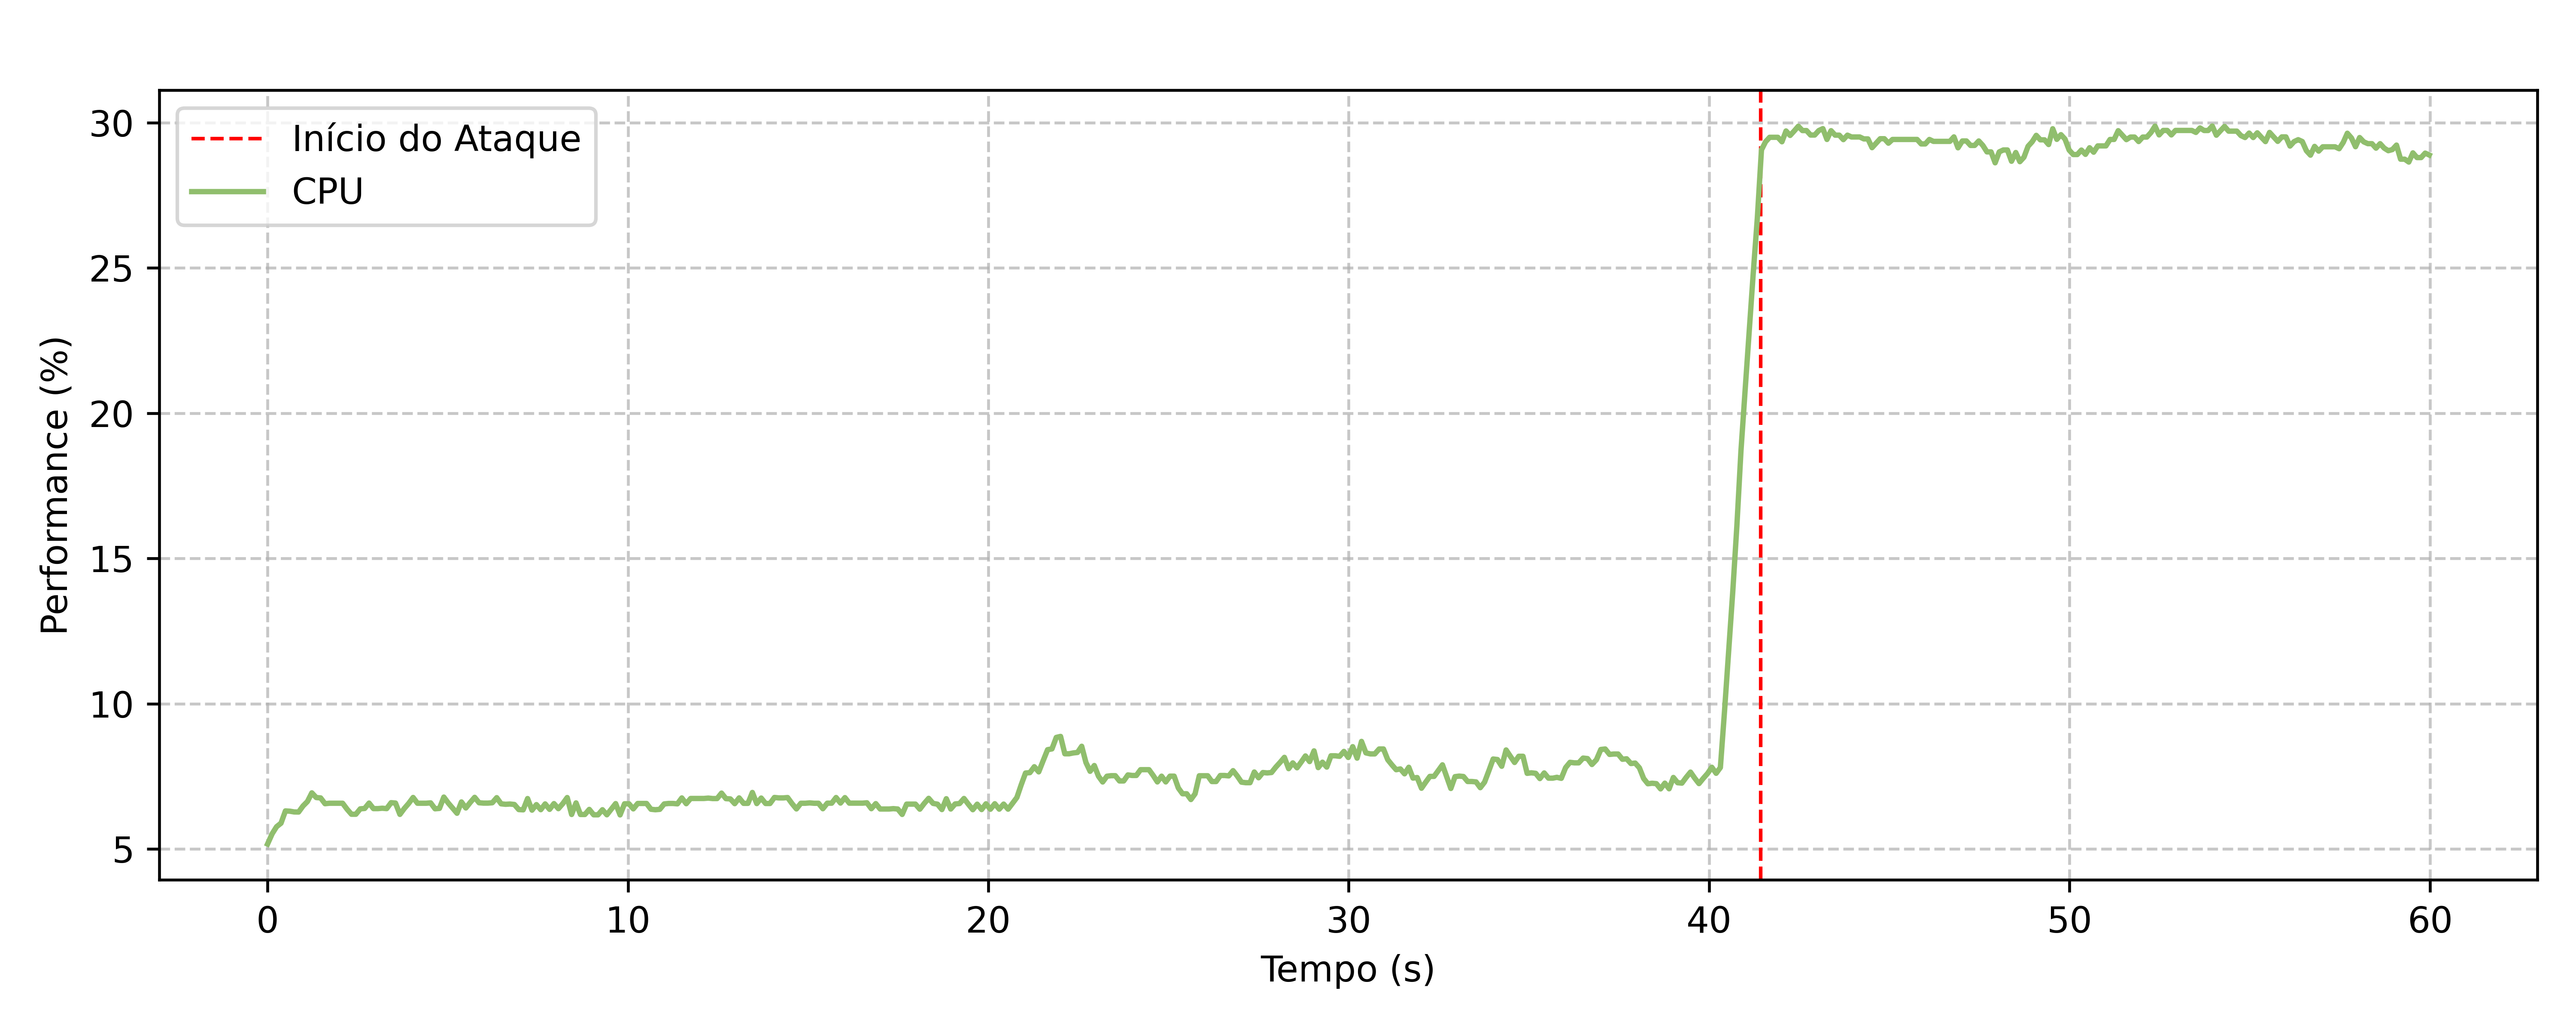
\includegraphics[width=1\textwidth]{USPSC-img/0-dos-hping-cpu.png}
                \end{subfigure}%
                \\
                \begin{subfigure}[t]{1\textwidth}
                    \centering
                    \caption{`Sign'}
                    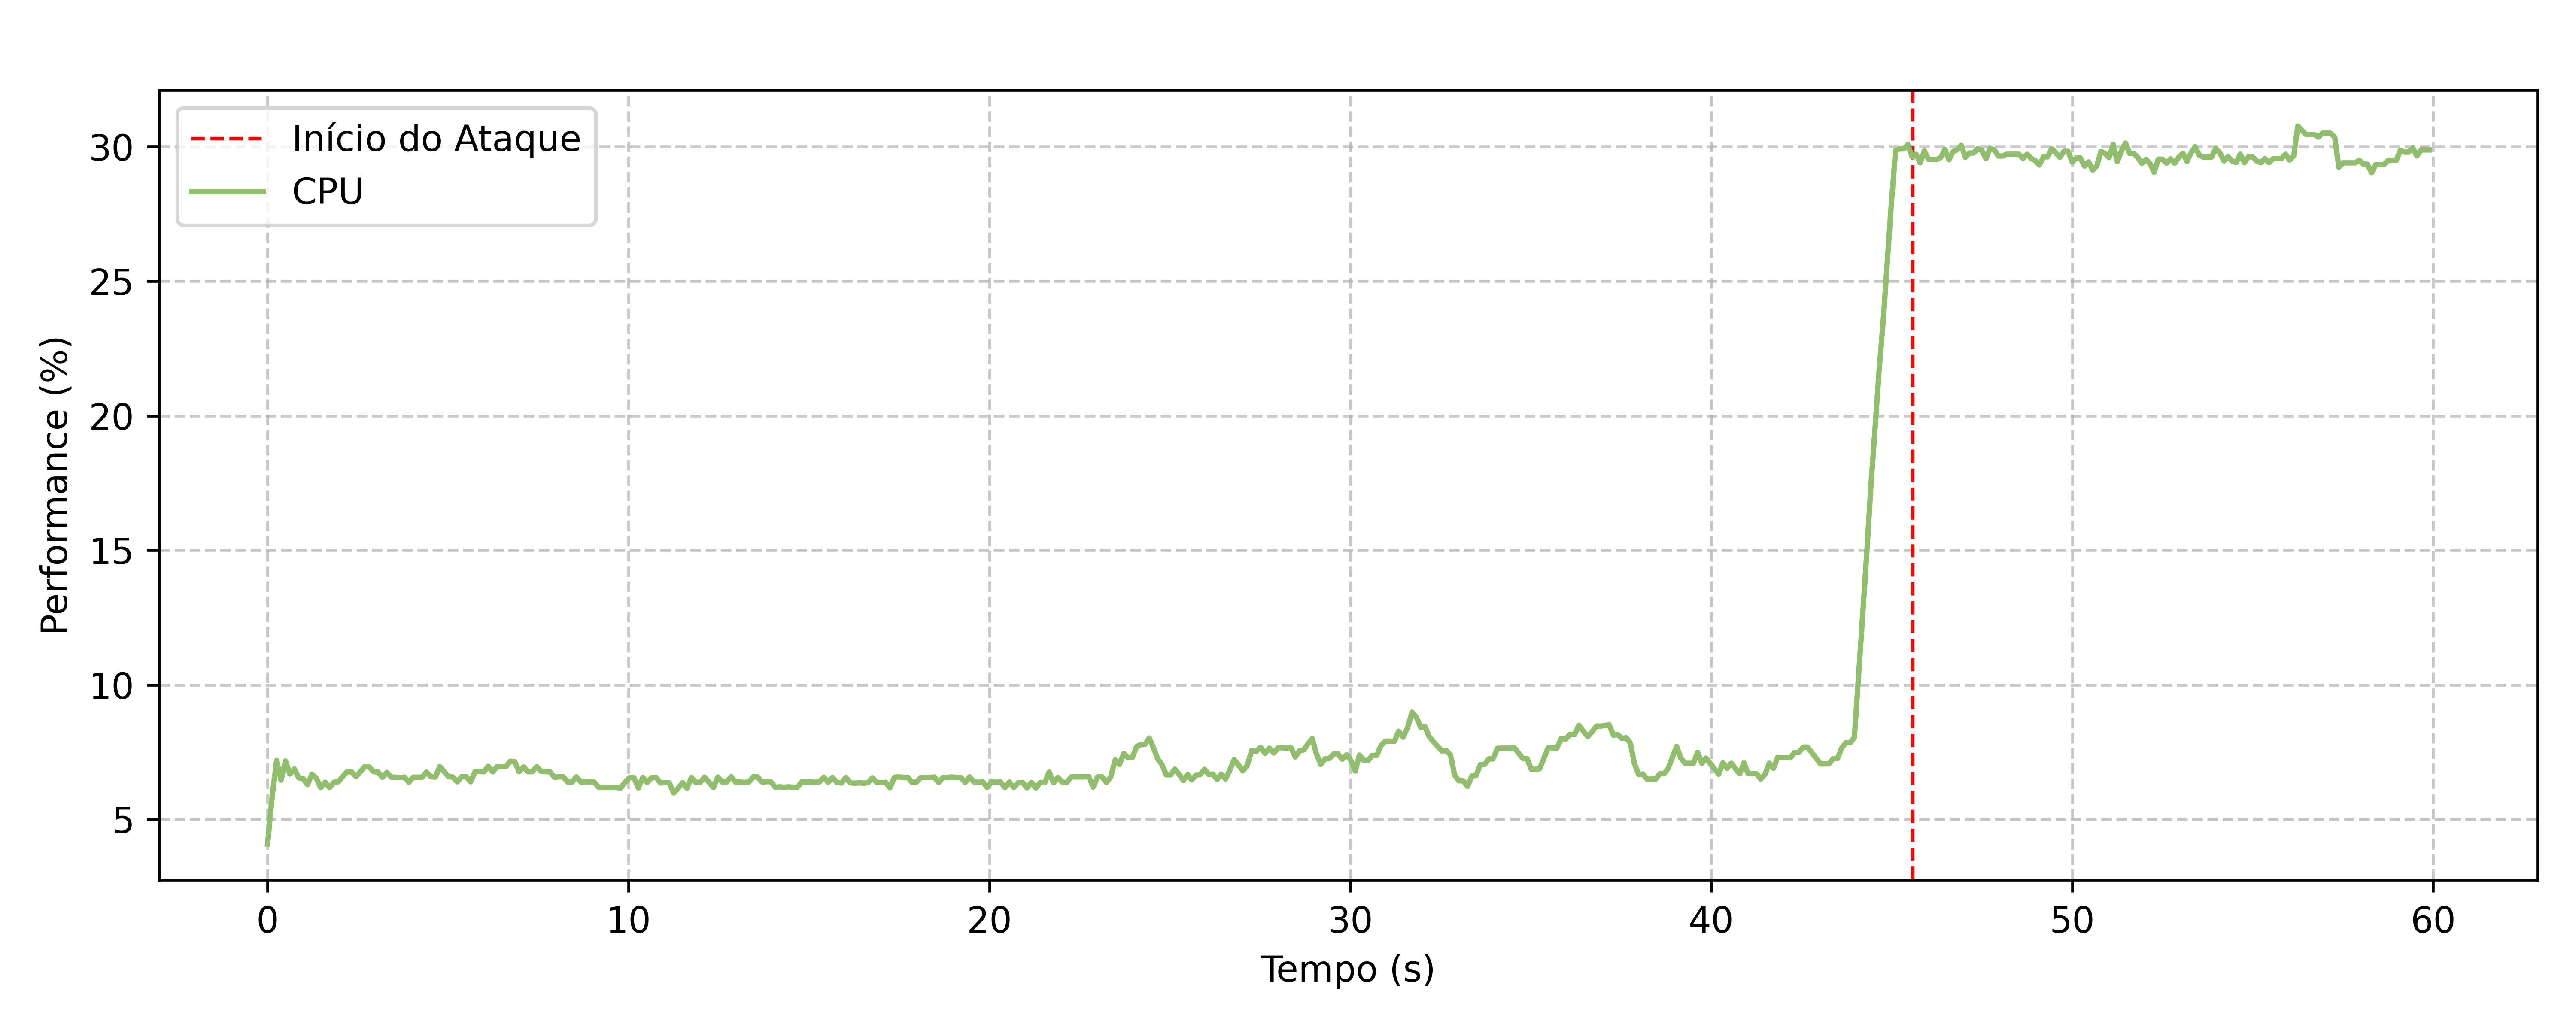
\includegraphics[width=1\textwidth]{USPSC-img/1-dos-hping-cpu.png}
                \end{subfigure}%
                \\
                \begin{subfigure}[t]{1\textwidth}
                    \centering
                    \caption{`Sign \& Encrypt'}
                    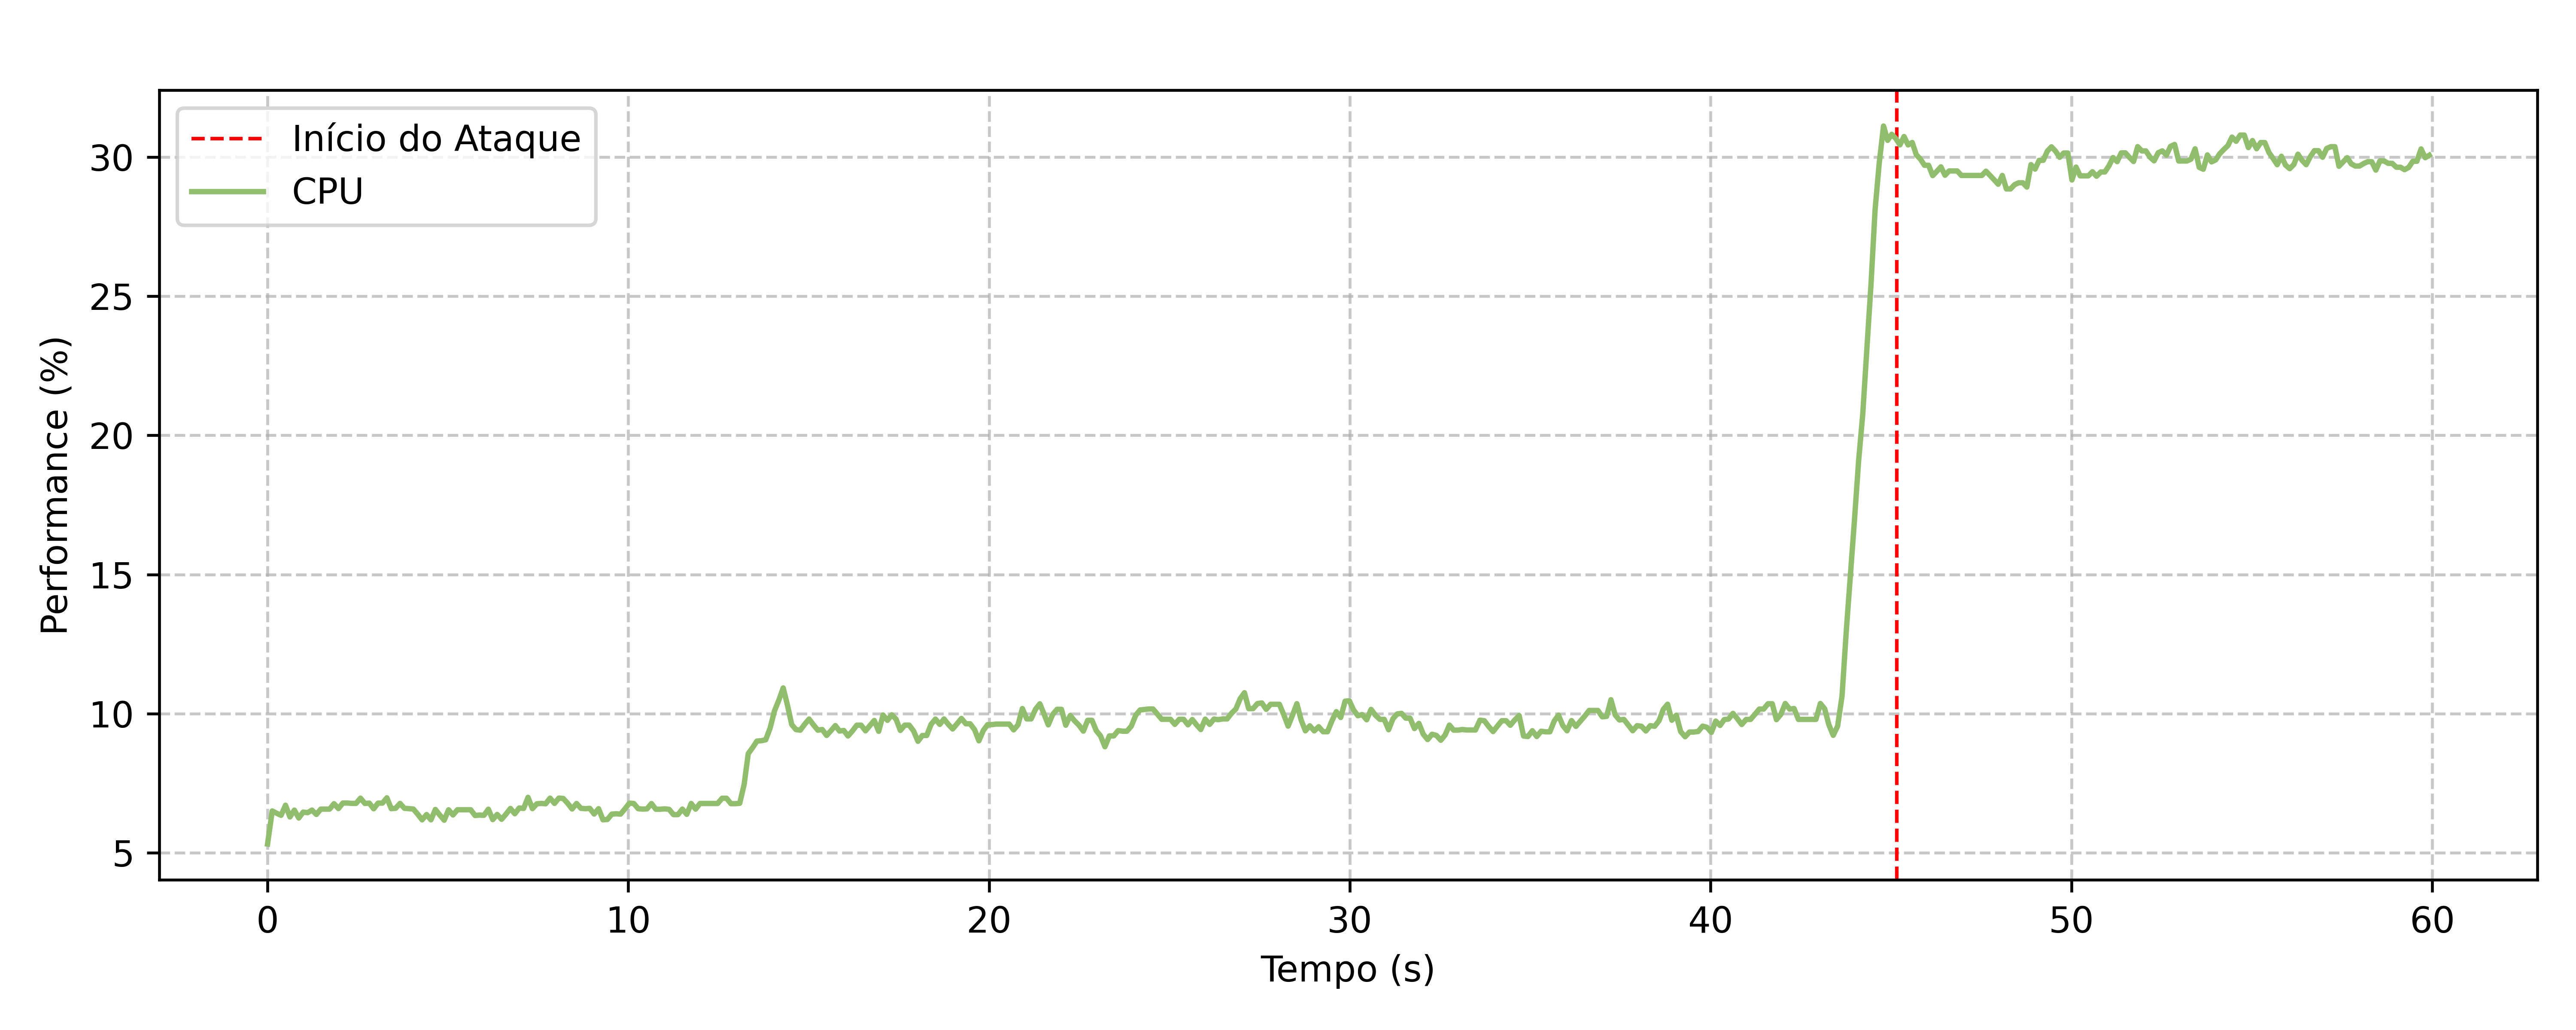
\includegraphics[width=1\textwidth]{USPSC-img/2-dos-hping-cpu.png}
                \end{subfigure}%
                \legend{Fonte: elaborada pelo autor.}
            \end{figure}

            Em média, o aumento de 275\% no uso do processamento no início do ataque, independentemente da configuração de segurança, indica que o servidor OPC UA é altamente vulnerável a ataques de inundação TCP/IP. Isso é evidenciado pelo fato de que os ataques foram executados em um ambiente controlado, onde nenhuma outra tarefa estava sendo processada pelo controlador. A alta carga de tráfego gerada por esse tipo de ataque pode levar à degradação do serviço, interrupção da comunicação e perda de dados críticos. Portanto, é essencial implementar medidas de segurança robustas para proteger a rede contra esse tipo de ataque, garantindo a disponibilidade e a integridade dos sistemas industriais.

            No entanto, é importante destacar que este ataque não foi direcionado especificamente ao protocolo OPC UA, mas sim à camada de transporte (quarta camada do modelo OSI). Embora a comunicação OPC UA não seja diretamente afetada, a corrupção da infraestrutura de rede subjacente pode ter impactos significativos na comunicação OPC UA, especialmente em ambientes industriais, onde a disponibilidade e a integridade dos sistemas são essenciais.

        \subsubsection*{\underline{Loop infinito na cadeia de certificados}}

            A tecnologia OPC UA demonstrou considerável resistência ao ataque de negação de serviço por loop infinito na cadeia de certificados. Essa análise pode ser realizada com base nos gráficos de RTT da comunicação. A Figura \ref{fig:0-dos-cert-rttp} apresenta a variação média do RTT normalizado por pacote durante a execução do ataque para o cenário C3.

            \begin{figure}[htbp!]
                \caption{\label{fig:0-dos-cert-rttp}Tempo de ida e volta normalizado por pacote durante o ataque de loop infinito na cadeia de certificados - nível de segurança: `Sign \& Encrypt'}
                \begin{center}
                    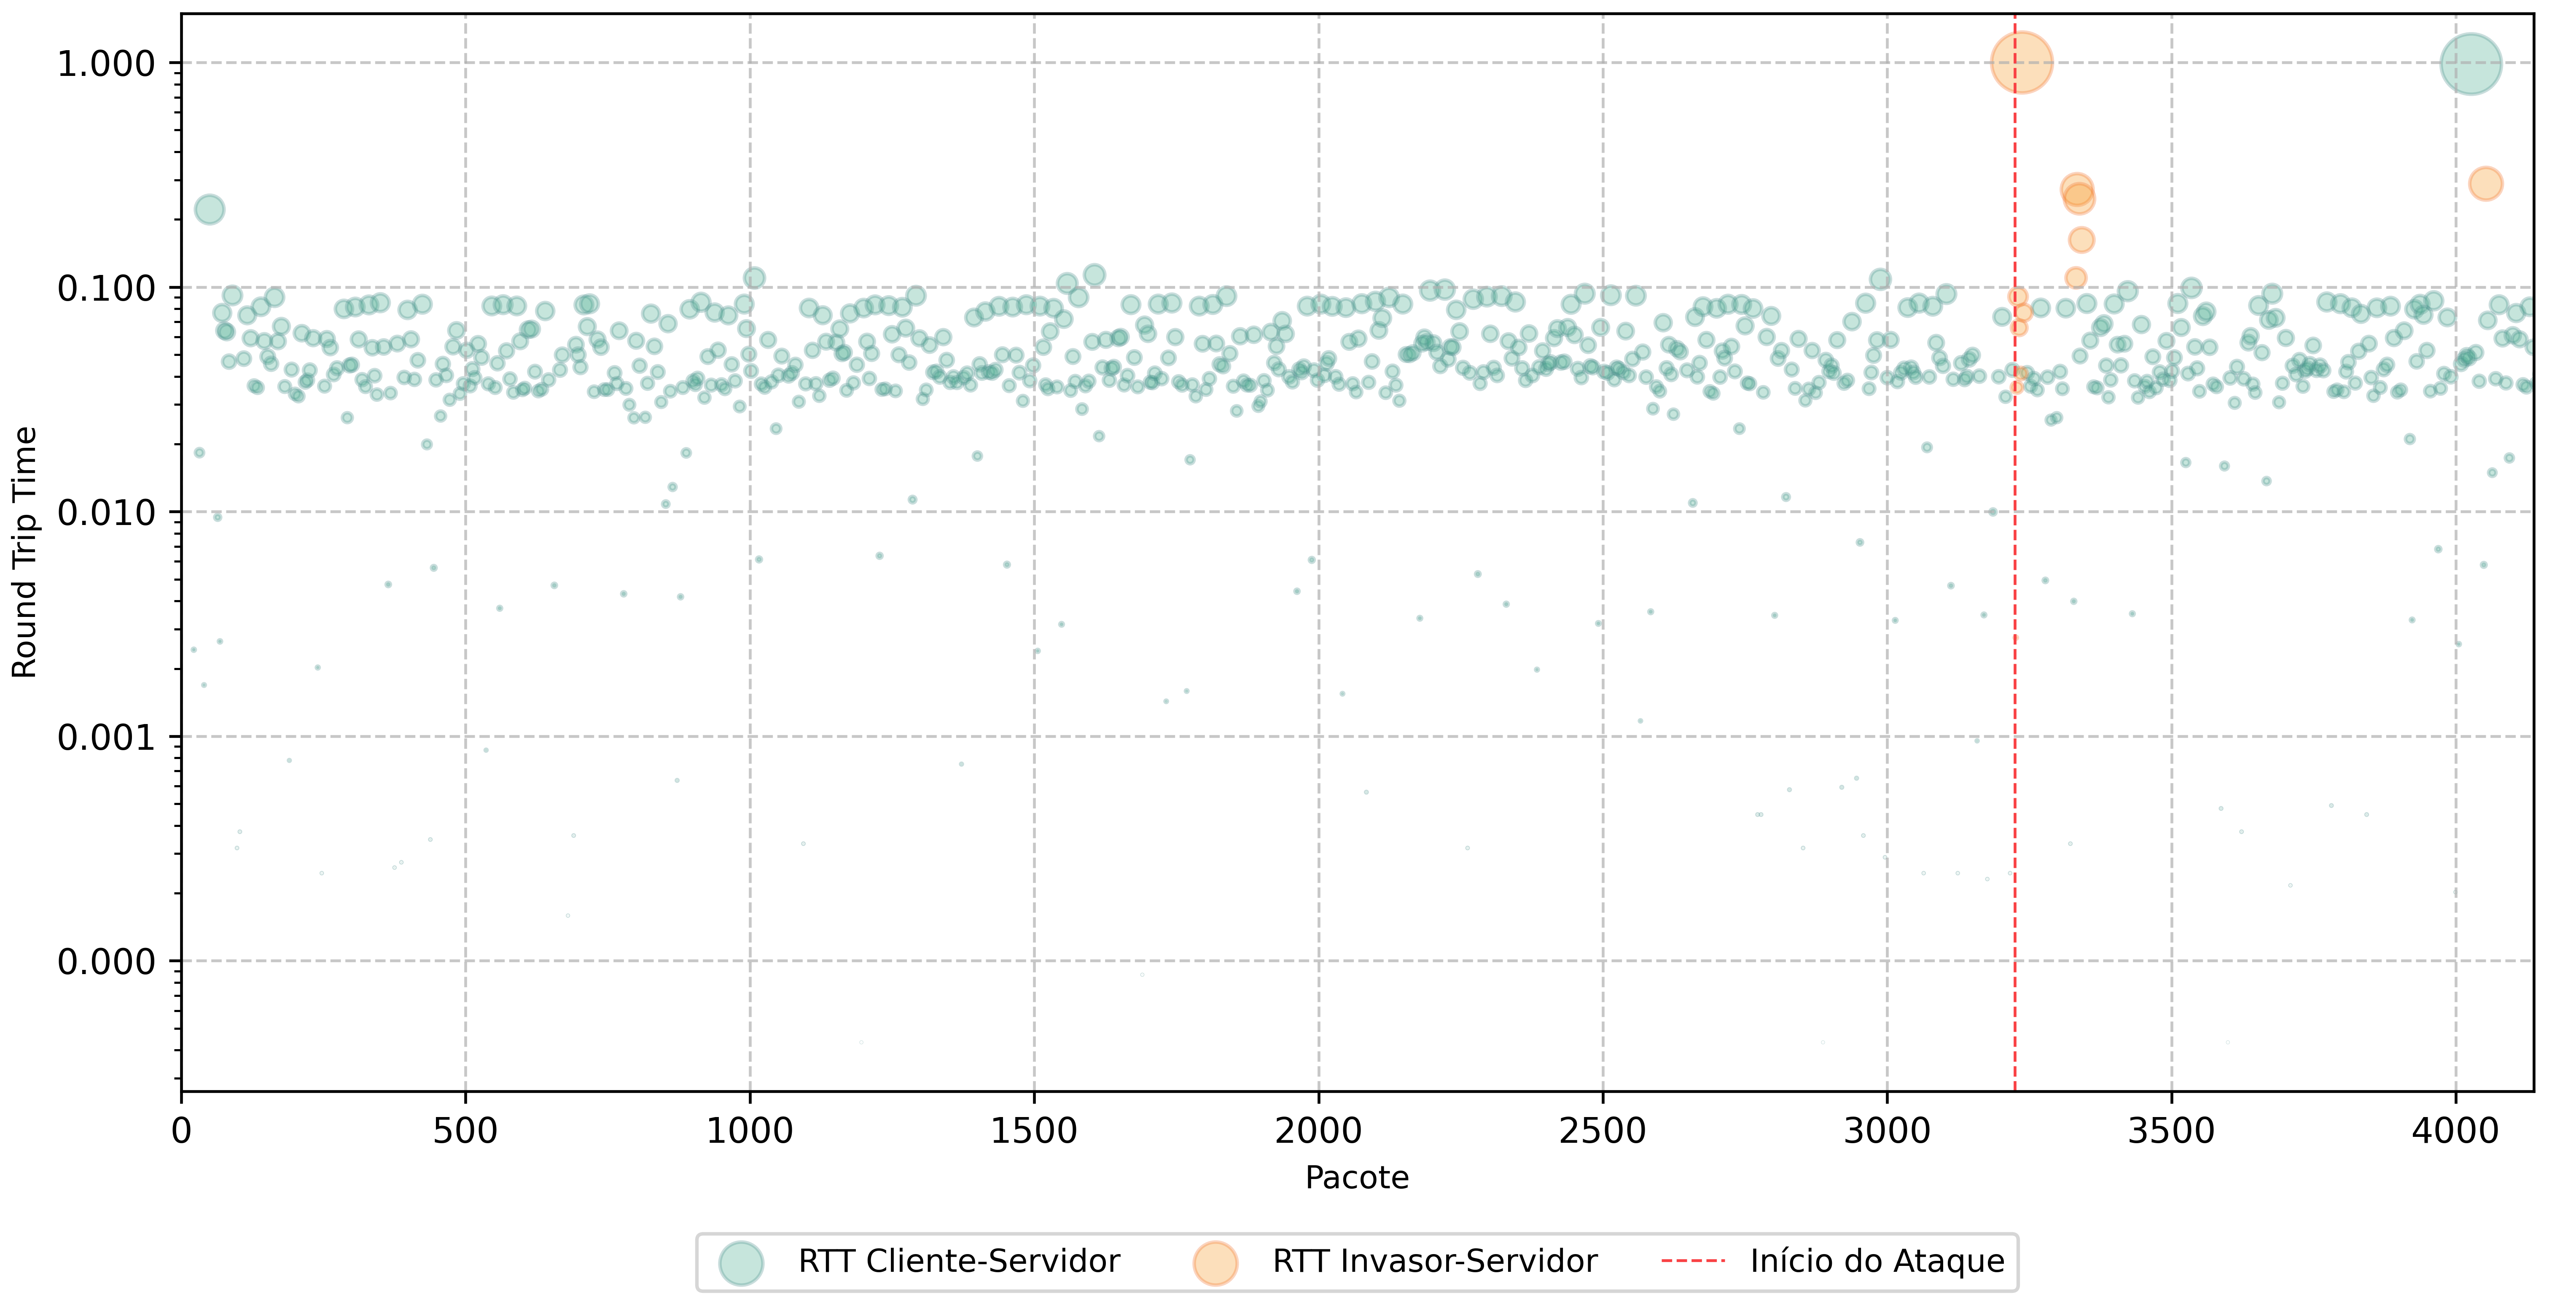
\includegraphics[width=0.972\textwidth]{USPSC-img/output/cropped/2-dos_certificate_inf_chain_loop-rttp.png}
                \end{center}
                \legend{Fonte: elaborada pelo autor.}
            \end{figure}

            A análise dos resultados revela que o invasor interage com o servidor OPC UA apenas no início do ataque. A comunicação é encerrada a partir desse ponto para todos os modos de segurança, conforme indicado pela linha vermelha pontilhada que marca o início do ataque. Antes do ataque, o RTT Cliente-Servidor se mantém constante e estável. No entanto, após o início do ataque, observa-se um aumento no RTT Invasor-Servidor, indicando que o servidor está sendo inundado com solicitações, o que resulta no aumento do tempo de resposta.

            O gráfico também revela que, após o início do ataque, há uma dispersão significativa dos valores de RTT Invasor-Servidor, sugerindo variações na capacidade do servidor de processar pacotes sob a carga do ataque. Entretanto, o RTT Cliente-Servidor apresenta pouca variação, indicando que o servidor consegue manter a qualidade do serviço para comunicações legítimas, apesar da sobrecarga causada pelo ataque.

            Essa análise reforça a eficácia do OPC UA em manter a resiliência contra ataques de negação de serviço, especialmente em cenários onde são implementadas medidas de segurança robustas, como o uso de criptografia e autenticação adequadas. Além disso, destaca a importância de monitorar continuamente o desempenho do servidor e de implementar mecanismos de mitigação de ataques para garantir a continuidade do serviço e a integridade dos dados.

        \subsubsection*{\underline{Chamada da função Dereference nula}}

            O ataque de DoS pela chamada da função Dereference nula revelou-se o único capaz de causar uma negação de serviço completa na rede OPC UA industrial, em todos os diferentes cenários (C4, C5 e C6). Esse ataque explora uma vulnerabilidade crítica no servidor, na qual uma chamada de função é executada sem verificar a validade do ponteiro, resultando em uma falha que pode travar o servidor. A técnica aproveita vulnerabilidades na desreferenciação de um ponteiro nulo, que ocorre quando um programa tenta acessar ou modificar um ponteiro que, em vez de apontar para uma localização válida na memória, possui um valor nulo. A consequência imediata é que o programa tenta ler ou escrever em uma área de memória inválida, levando a uma interrupção abrupta do funcionamento do sistema. A gravidade dessa falha reside no fato de que, além de interromper o serviço, ela pode ser explorada por atacantes para comprometer a segurança e a integridade do sistema, explorando comportamentos indefinidos que podem permitir a execução de código malicioso ou levar à negação de serviço, como neste caso.

            A análise dos gráficos fornecidos pela \autoref{fig:2-dos_null_deref} oferece uma compreensão detalhada do impacto desse ataque, especificamente para a rede configurada com modo de segurança `Sign \& Encrypt'.

            \begin{figure}[htbp!]
                \centering
                \caption{\label{fig:2-dos_null_deref}Gráficos do ataque de DoS pela chamada da função \textit{Dereference} nula - nível de segurança: `Sign \& Encrypt'.}
                \begin{subfigure}[t]{0.5\textwidth}
                    \centering
                    \caption{\label{fig:2-dos_null_deref-tput}\textit{Throughput}}
                    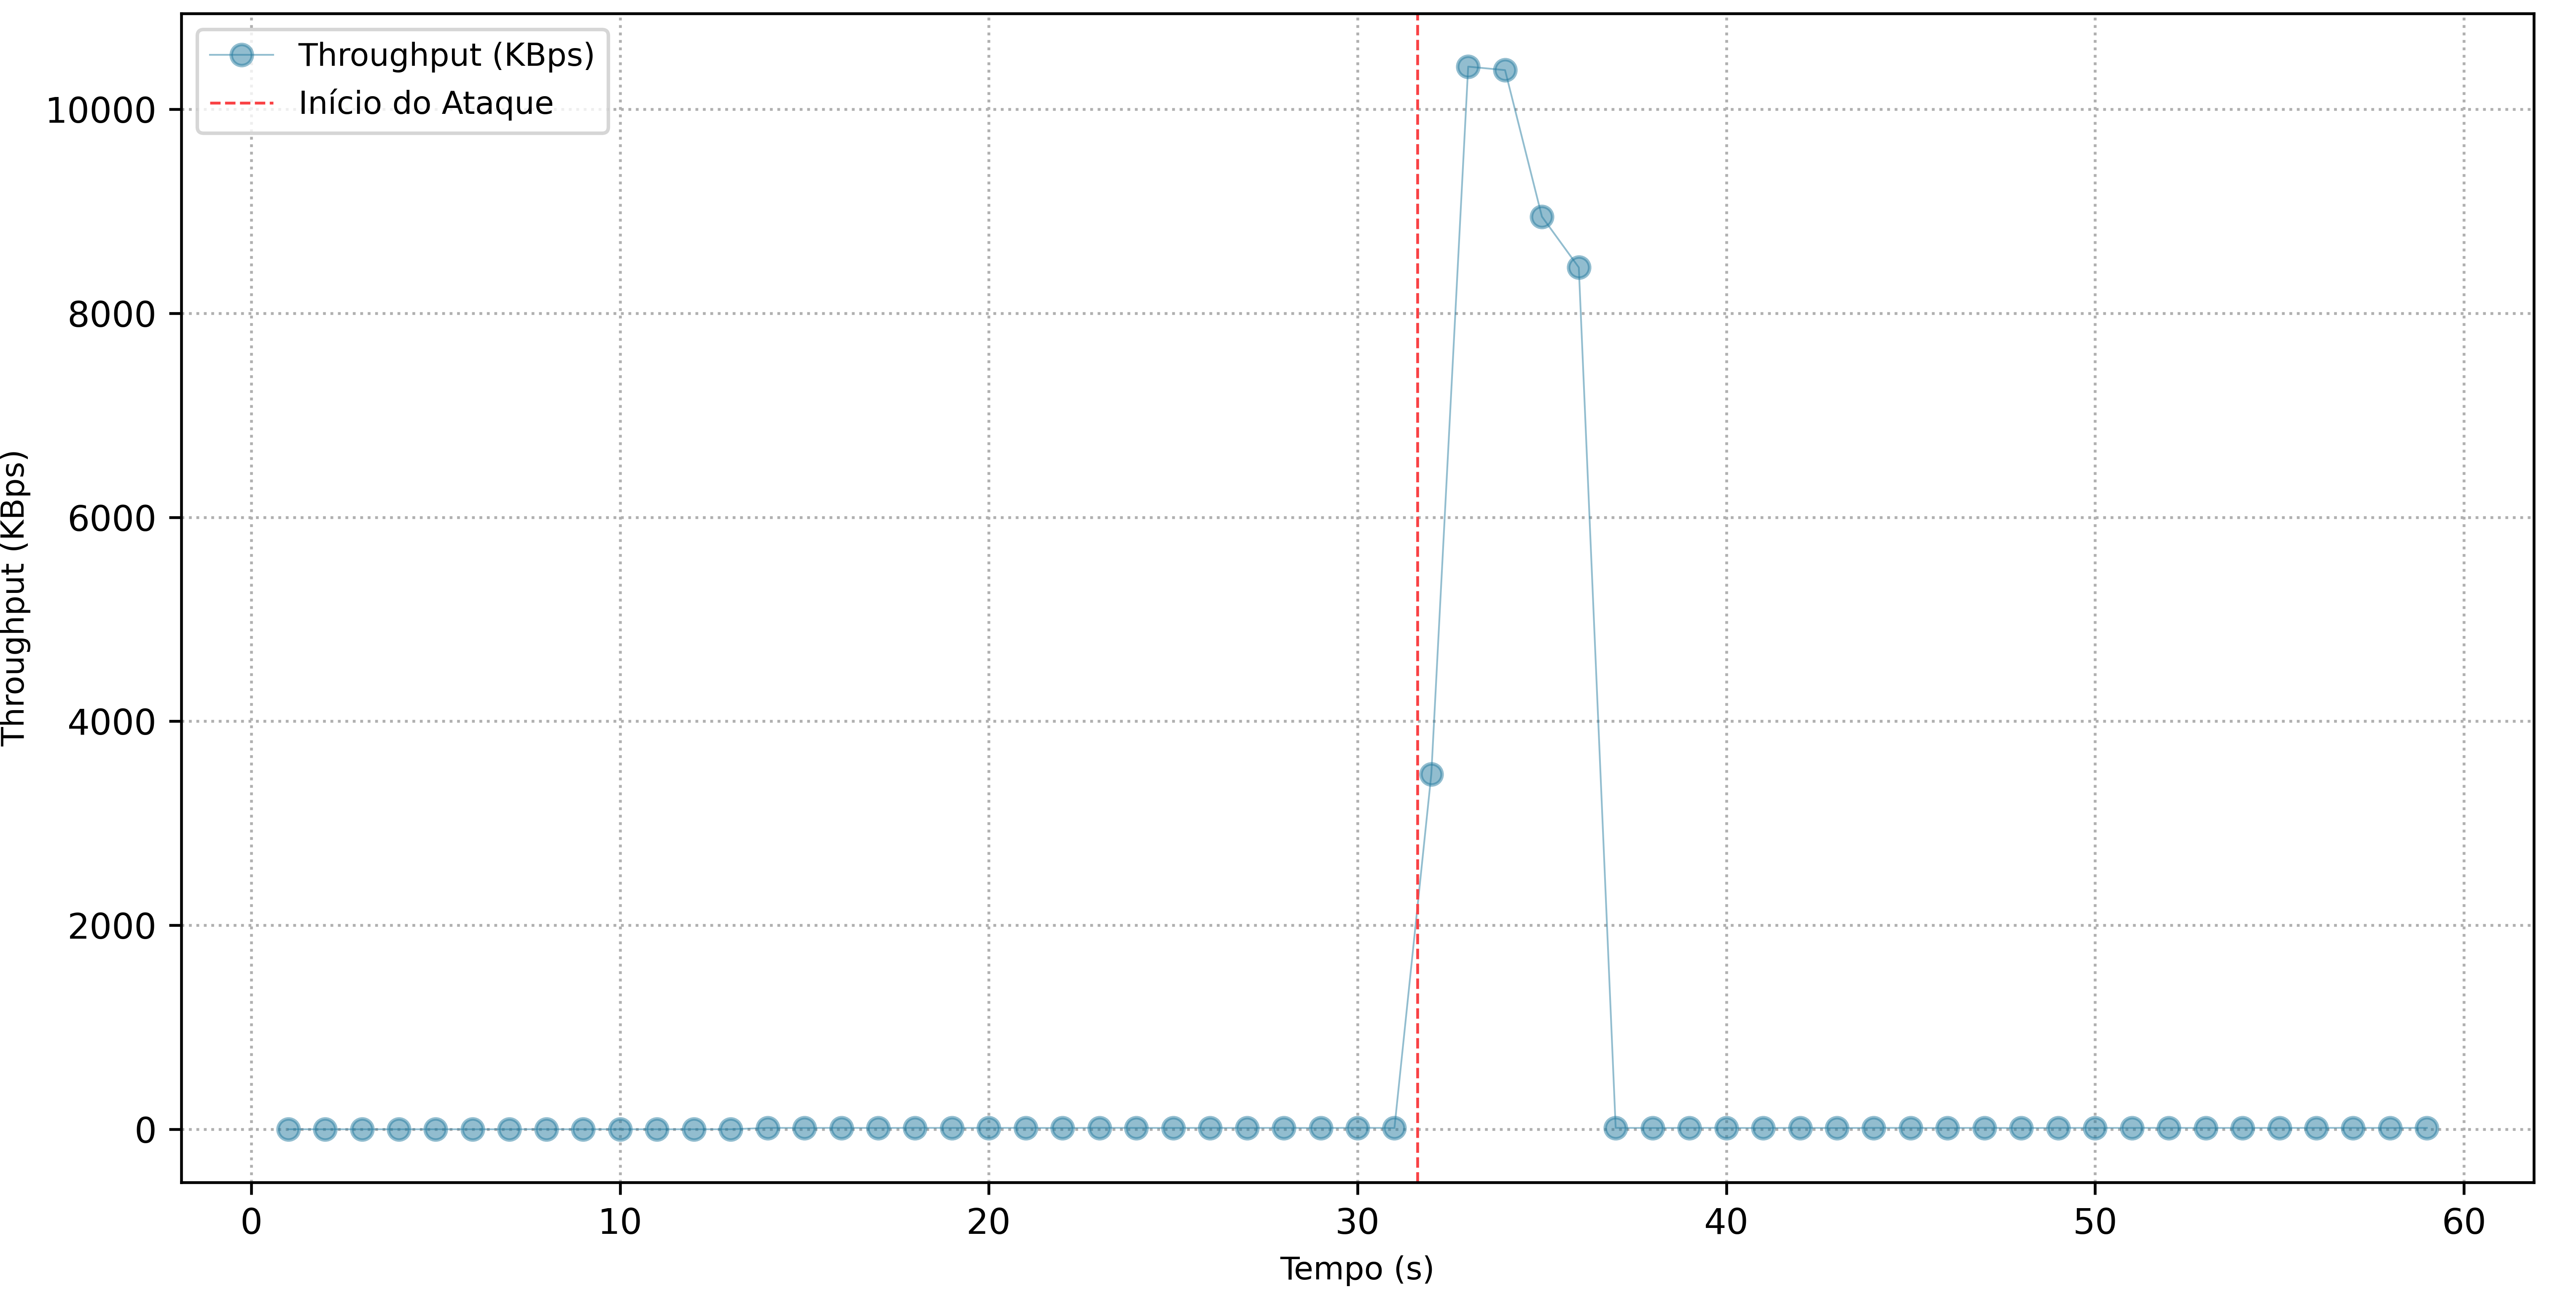
\includegraphics[width=1\textwidth, height=120pt]{USPSC-img/output/cropped/2-dos_function_call_null_deref-tput.png}
                \end{subfigure}%
                ~ 
                \begin{subfigure}[t]{0.5\textwidth}
                    \centering
                    \caption{\label{fig:2-dos_null_deref-perf}Desempenho}
                    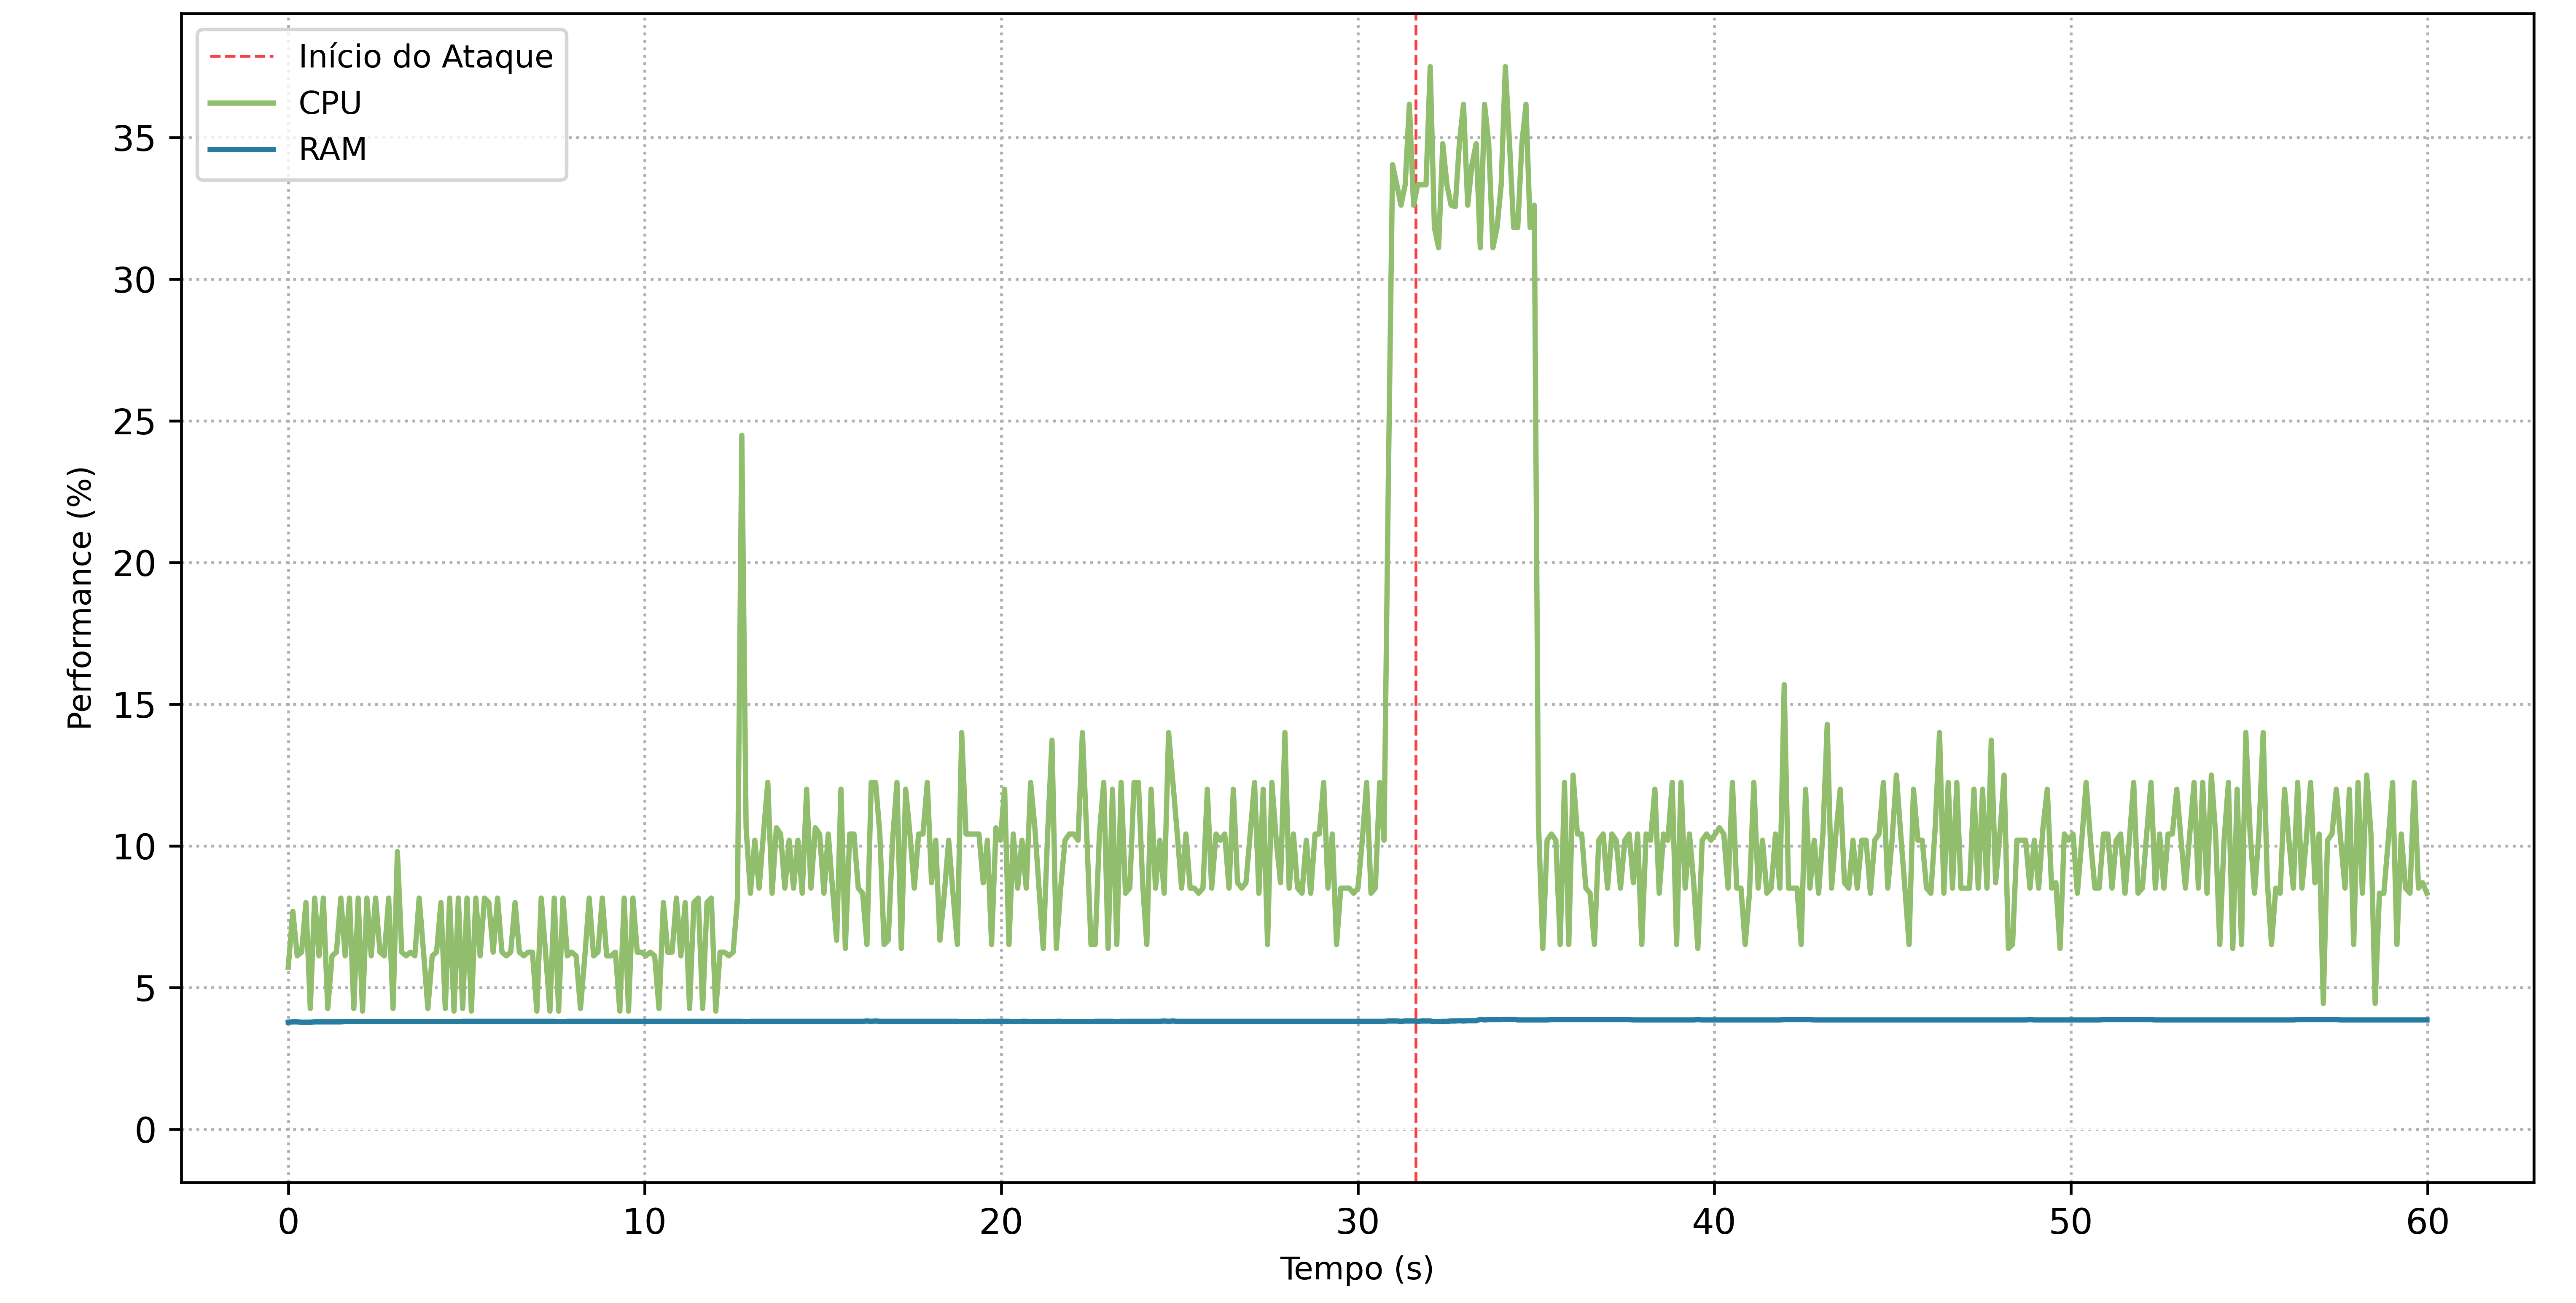
\includegraphics[width=1\textwidth, height=120pt]{USPSC-img/output/cropped/2-dos_function_call_null_deref-perf.png}
                \end{subfigure}%
                \\
                \begin{subfigure}[t]{0.5\textwidth}
                    \centering
                    \caption{\label{fig:2-dos_null_deref-pack}Pacotes OPC UA}
                    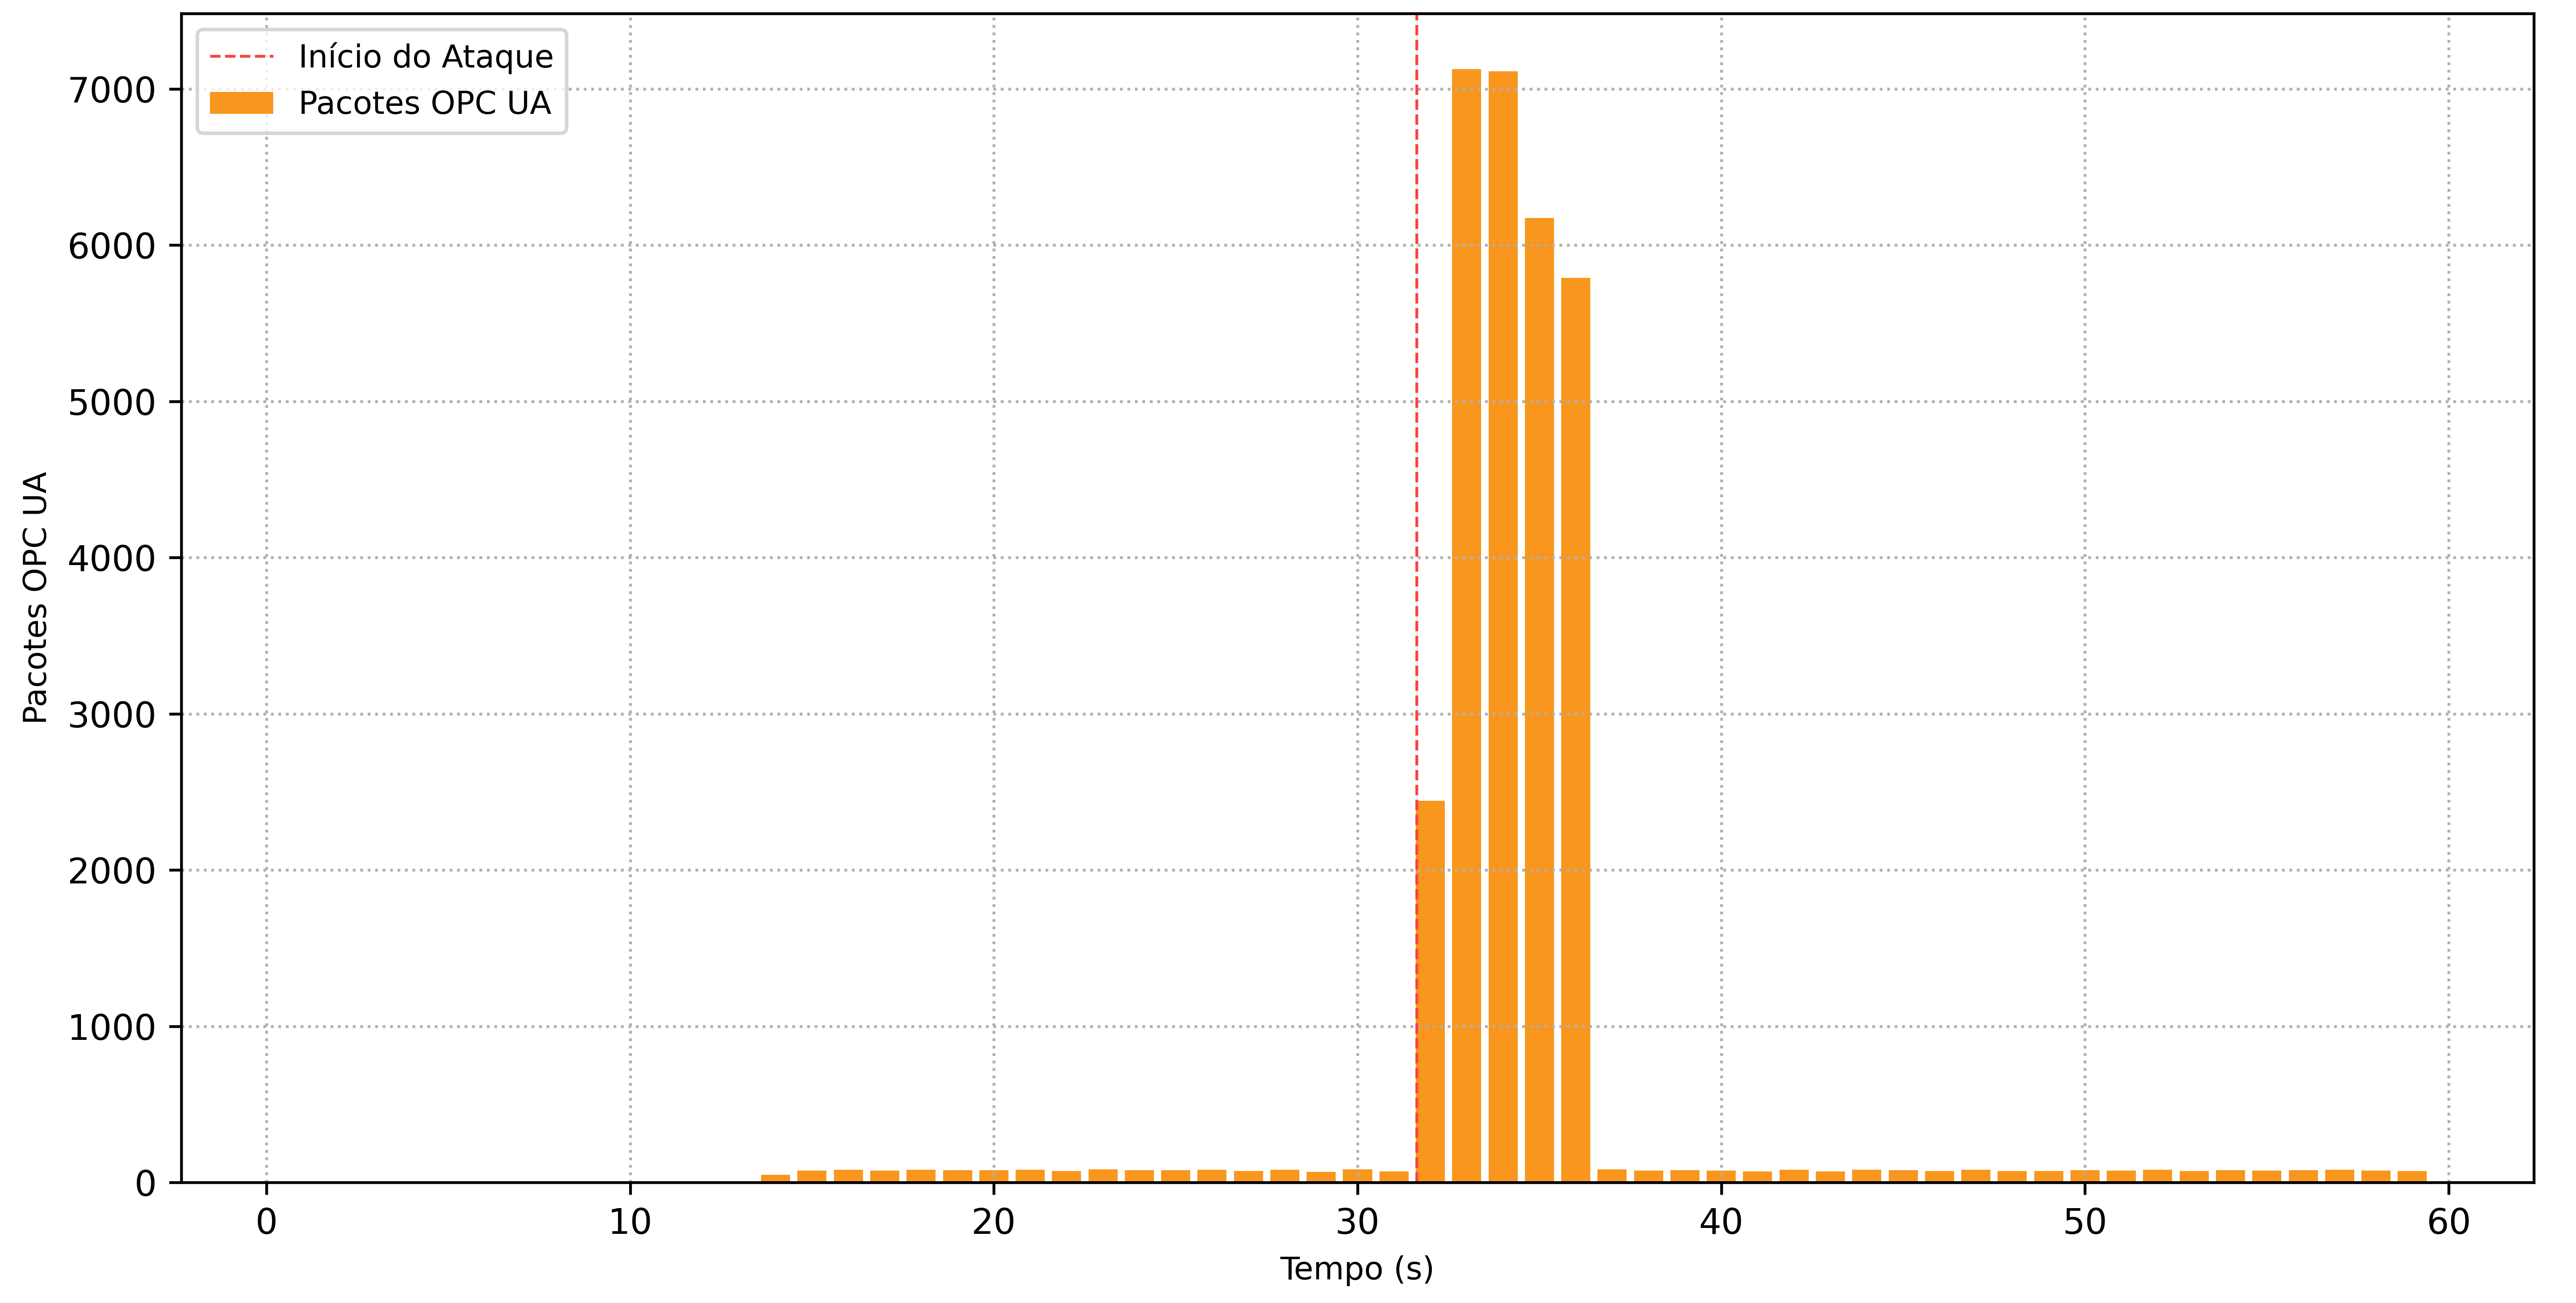
\includegraphics[width=1\textwidth, height=120pt]{USPSC-img/output/cropped/2-dos_function_call_null_deref-pack.png}
                \end{subfigure}%
                ~
                \begin{subfigure}[t]{0.5\textwidth}
                    \centering
                    \caption{\label{fig:2-dos_null_deref-rttp}RTT por pacote}
                    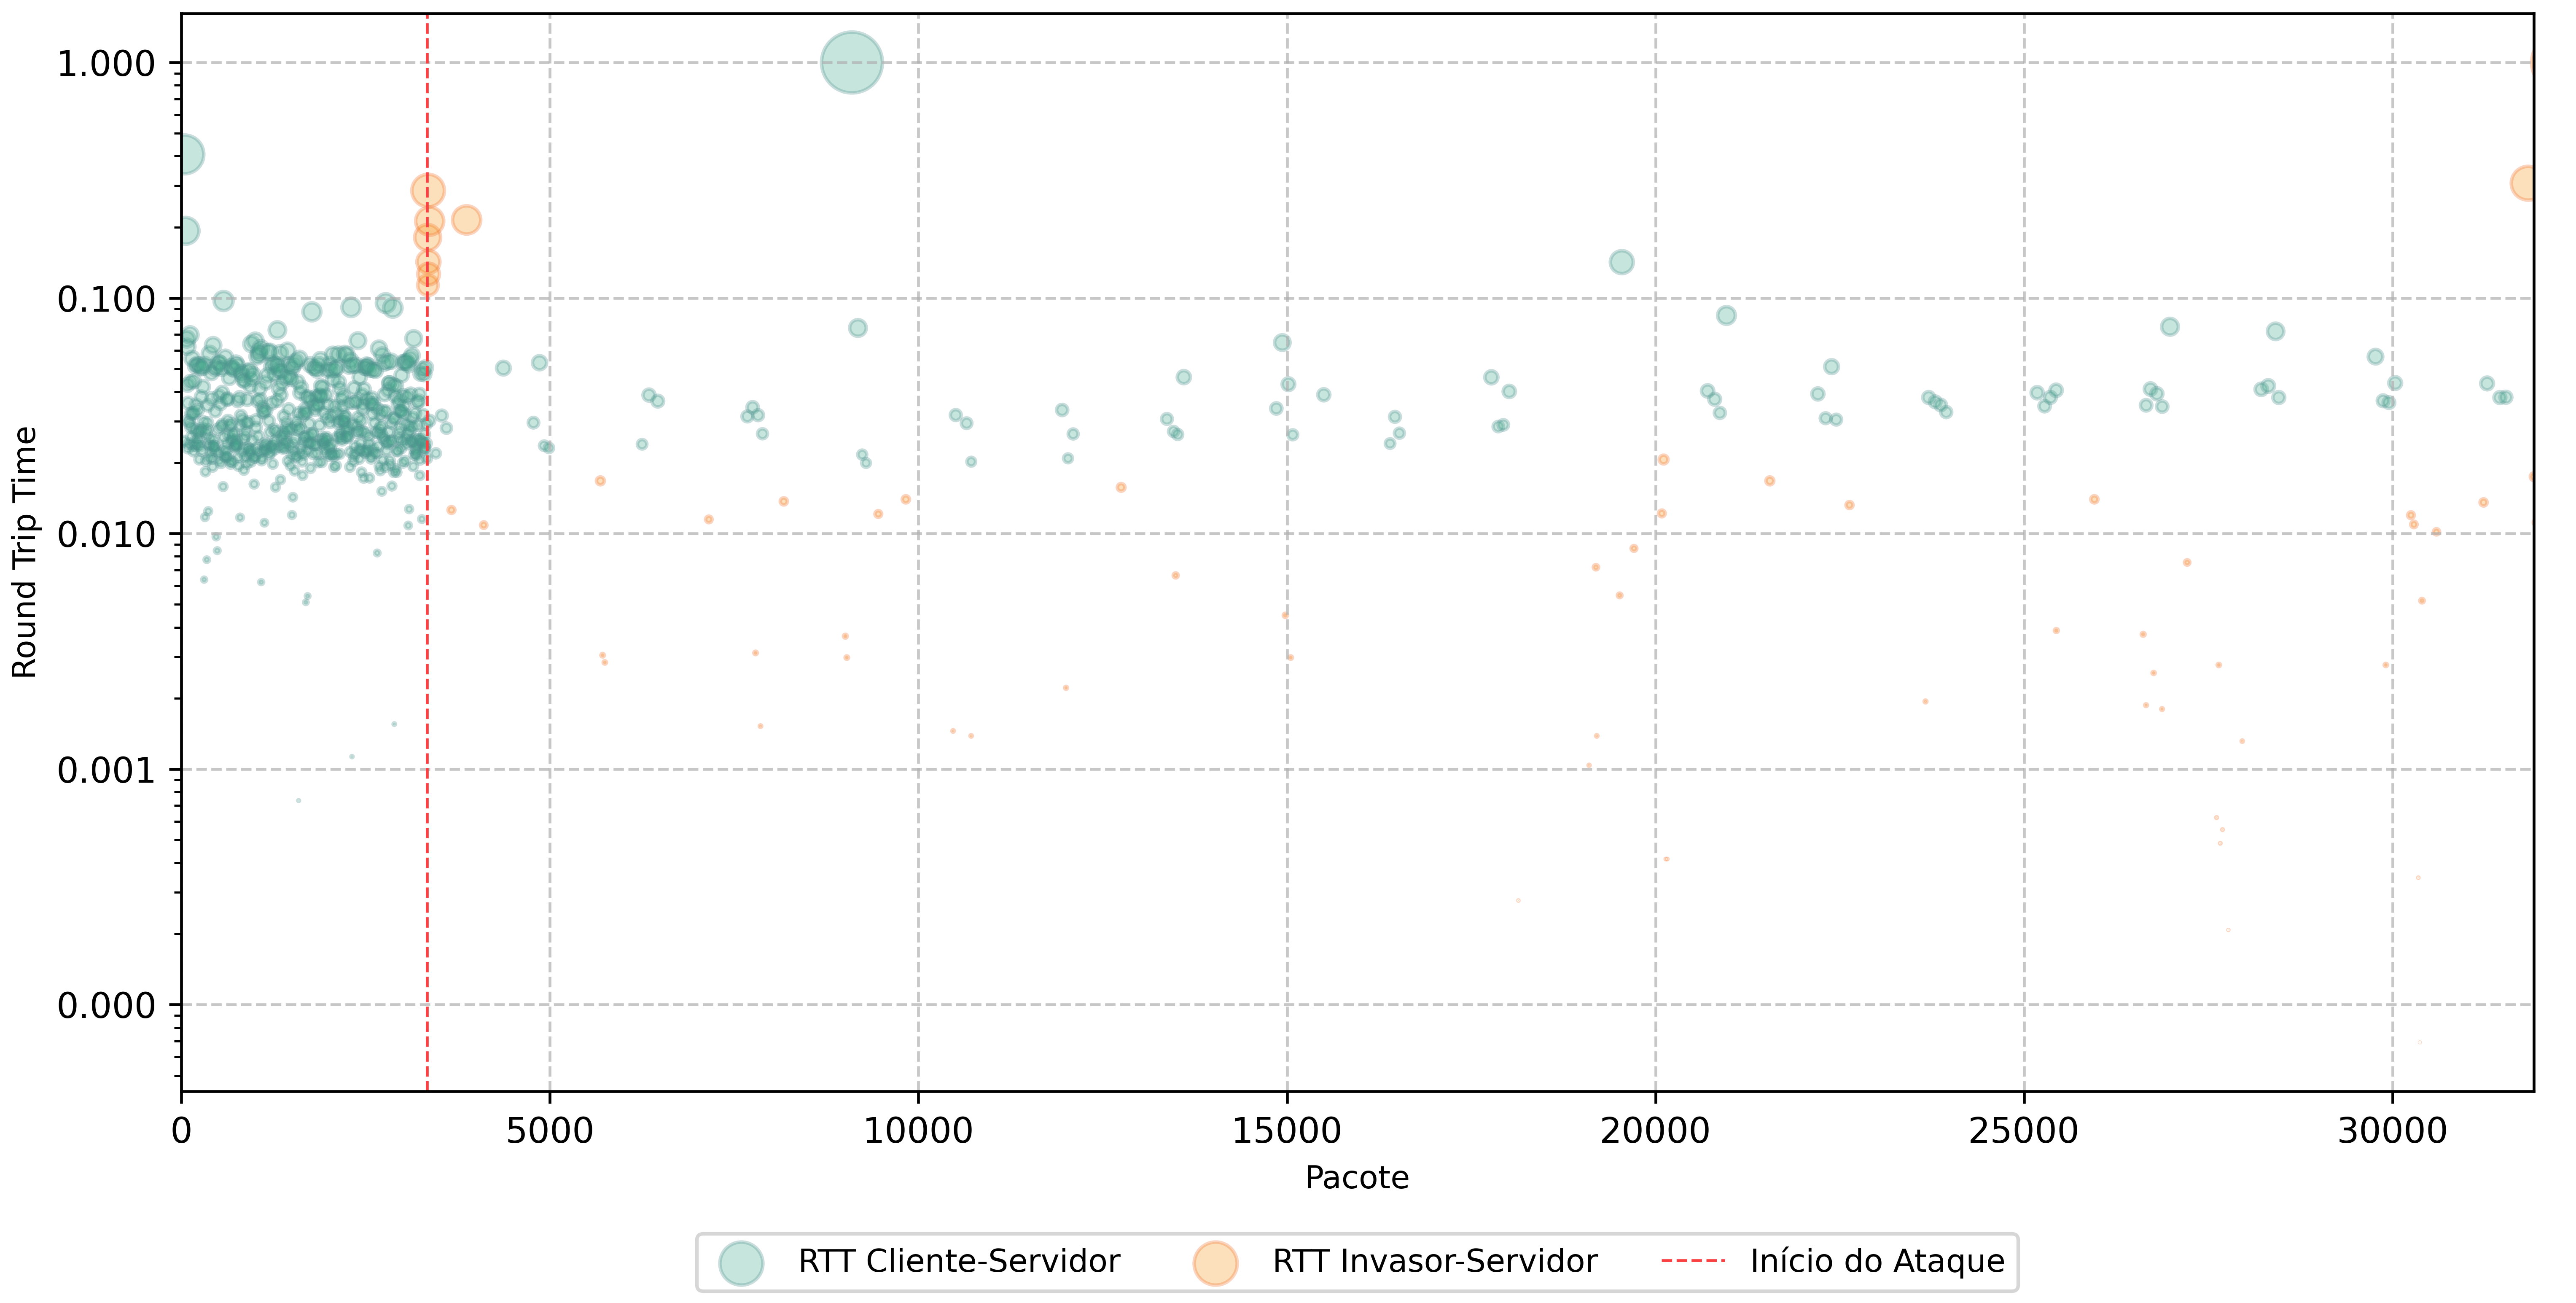
\includegraphics[width=1\textwidth, height=120pt]{USPSC-img/output/cropped/2-dos_function_call_null_deref-rttp.png}
                \end{subfigure}%
            \end{figure}

            O gráfico de taxa de transferência, representado na \autoref{fig:2-dos_null_deref-tput}, demonstra uma estabilidade em níveis baixos antes do ataque. Com o início do ataque, indicado pela linha vermelha, observa-se um aumento abrupto no \textit{throughput}, atingindo um pico significativo antes de cair drasticamente a zero. Esse comportamento indica que o servidor OPC UA foi sobrecarregado com solicitações inválidas, resultando em uma falha completa da comunicação, o que caracteriza uma negação de serviço.

            A análise do gráfico de tempo de ida e volta por pacote, ilustrado na \autoref{fig:2-dos_null_deref-rttp}, corrobora esses achados. Antes do ataque, o RTT entre cliente e servidor permanece relativamente constante, refletindo uma comunicação estável. No entanto, com o início do ataque, há um aumento significativo no RTT, especialmente na comunicação entre o invasor e o servidor. Essa elevação súbita no RTT sugere que o servidor está demorando mais para processar as solicitações devido à sobrecarga provocada pelo ataque, culminando em um colapso na comunicação.

            O impacto do ataque na performance do servidor é ainda mais evidente na \autoref{fig:2-dos_null_deref-perf}, que mostra o desempenho do host em termos de utilização de CPU e memória RAM. Antes do ataque, o uso da CPU se mantém em níveis baixos e constantes, indicando um funcionamento normal do servidor. Todavia, após o início do ataque, a utilização da CPU aumenta drasticamente, enquanto a utilização da RAM permanece estável. Essa alta utilização da CPU é um indicativo claro de que o servidor está sobrecarregado tentando processar a grande quantidade de solicitações inválidas geradas pelo ataque, levando a uma queda de desempenho e, eventualmente, à falha do sistema.

            Esses resultados demonstram que o ataque de chamada da função de desreferenciação nula é altamente eficaz em explorar vulnerabilidades específicas do servidor OPC UA, resultando em uma negação de serviço completa. A incapacidade do servidor de verificar a validade dos ponteiros antes de executar chamadas de funções críticas foi o fator chave que permitiu a execução bem-sucedida desse ataque. A rápida elevação na utilização da CPU e a subsequente falha na comunicação destacam a necessidade urgente de medidas de mitigação para proteger servidores OPC UA contra tais vulnerabilidades.

        \subsubsection*{\underline{Abertura de múltiplos canais seguros}}

            A análise dos ataques de DoS por meio de solicitações de abertura de múltiplos canais seguros na comunicação OPC UA revela uma vulnerabilidade crítica com potencial para comprometer redes industriais. O ataque explora a limitação do servidor OPC UA em gerenciar simultaneamente essas requisições, resultando em sobrecarga e eventual interrupção do serviço.

            Os resultados dos experimentos demonstram que a abertura simultânea de múltiplos canais seguros pode levar a um aumento significativo no \textit{throughput}, no tempo de resposta e na utilização da CPU. A \autoref{fig:0-dos-open-tput} mostra que, logo após o início do ataque, o servidor tenta lidar com o excesso de requisições, mas sua capacidade de processamento se revela insuficiente para manter a eficiência, resultando em sobrecarga. Proporcionalmente, observam-se efeitos adversos substanciais no RTT e no desempenho do host após o início do ataque.

            \begin{figure}[htbp!]
                \caption{\label{fig:0-dos-open-tput}Taxa de transferência durante o ataque de abertura de múltiplos canais seguros - nível de segurança: `Sign'}
                \begin{center}
                    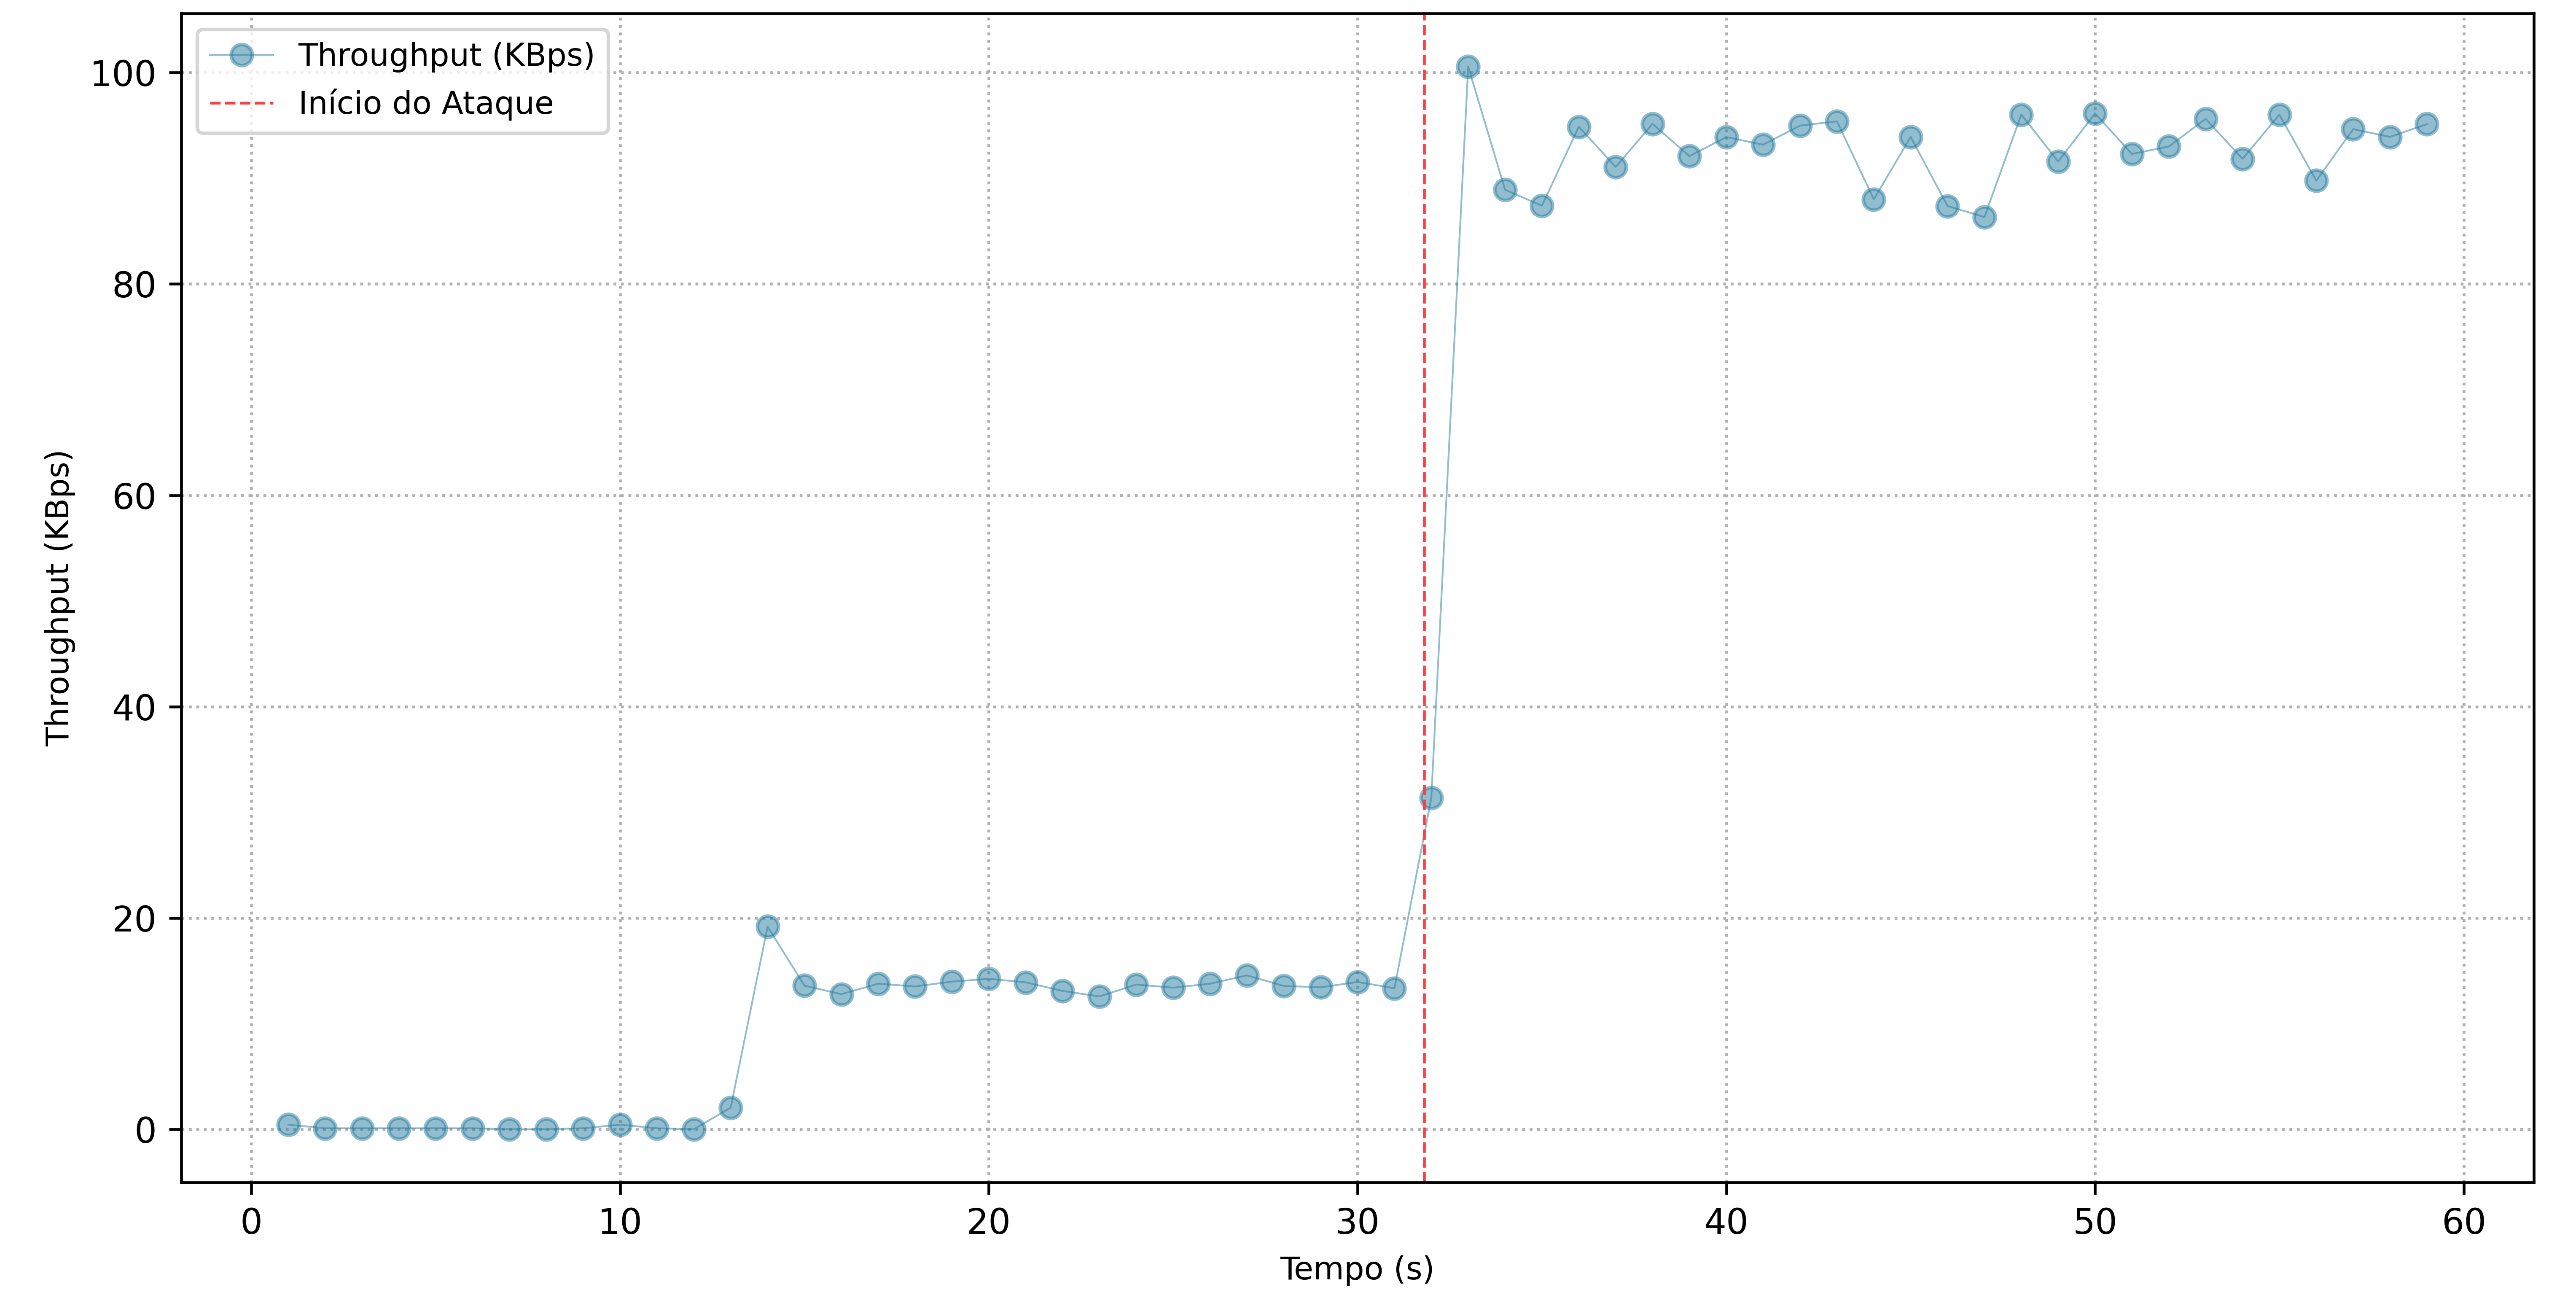
\includegraphics[width=0.972\textwidth]{USPSC-img/output/cropped/1-dos_open_multiple_secure_channels-tput.png}
                \end{center}
                \legend{Fonte: elaborada pelo autor.}
            \end{figure}

        \subsubsection*{\underline{Tradução do caminho de navegação}}

            Uma vulnerabilidade crítica que pode ser explorada para comprometer a estabilidade e a segurança da rede OPC UA é a exaustão da pilha de função que processa requisições de tradução de caminhos de navegação para \texttt{NodeIds} (\texttt{TranslateBrowsePathsToNodeIds}). A função \texttt{TranslateBrowsePath} é responsável por traduzir caminhos de navegação (do inglês \textit{browse paths}) em \texttt{NodeIds}. Durante esse processo, a função é chamada recursivamente para cada elemento no caminho relativo (\texttt{RelativePath}), sem um limite adequado para a profundidade da recursão. Como resultado, a tradução de um caminho de navegação excessivamente longo pode levar a uma exceção de estouro de pilha (\texttt{StackOverflowException}).

            Entretanto, a análise dos resultados obtidos para os cenários C13, C14 e C15 revela que a rede OPC UA apresenta uma leve proteção contra ataques de negação de serviço por exaustão da pilha de função. A análise dos gráficos de dados do tráfego da rede, especialmente o tempo de resposta do servidor, indica uma degradação significativa no desempenho do sistema ao longo do tempo, com um aumento acentuado à medida que o número de requisições maliciosas foi incrementado.

\section{Propostas de Melhorias e Mitigações} \label{sec:melhorias-mitigacoes}

    A melhoria da resiliência cibernética de um IACS deve ser um dos principais benefícios obtidos com a implementação de um programa de segurança industrial. Essa resiliência é alcançada quando os controles de segurança são selecionados de modo a abranger um processo contínuo de abordagem à cibersegurança, que não apenas se inicia com a dissuasão e prevenção de ameaças, mas também equilibra de forma adequada a detecção e correção de incidentes. Essa manobra gerencial é essencial para identificar eventos cibernéticos de maneira oportuna e responder adequadamente, a fim de minimizar as consequências e restaurar a operação normal da instalação de manufatura.

    As organizações frequentemente destinam grandes partes de seu orçamento de segurança a mecanismos de prevenção de ataques. No entanto, muitas vezes são alertadas por partes externas sobre a falta de investimento equilibrado em controles de detecção de incidentes, muito tempo após a ocorrência de um ataque. A segurança deve ser considerada um investimento estratégico de longo prazo, em vez de uma despesa tática de curto prazo ou isolada. Aqueles que investem e constroem instalações de manufatura compreendem o ciclo de vida de longo prazo do investimento de capital, por isso faz sentido que a segurança industrial destinada a proteger essas mesmas instalações seja tratada de maneira semelhante, recebendo atenção contínua (e orçamento) como outras despesas operacionais (manutenção, melhorias, treinamento, etc.).

    Nesta seção, são apresentadas as propostas de melhorias e mitigações identificadas, divididas em duas categorias principais: as recomendações para comunicações seguras com o protocolo OPC UA e as melhorias na infraestrutura e gestão de redes. Adicionalmente, na última subsessão, são descritas as normas e regulamentos que podem ser utilizados para garantir a conformidade com os requisitos de segurança industrial. Ao implementar essas recomendações, espera-se não apenas aumentar a robustez das comunicações, mas também assegurar a continuidade das operações industriais de forma segura e eficiente.

    \subsection{Recomendações para Comunicações Seguras com o Protocolo OPC UA}

        Especialmente no contexto do uso do protocolo OPC UA, uma série de testes realizados em conformidade com os padrões de segurança identificaram diversas recomendações visando mitigar vulnerabilidades e fortalecer tanto a integridade e a disponibilidade quanto a confidencialidade dos dados.

        Em primeiro lugar, assim como qualquer outro software ou protocolo, a atualização regular é crucial para manter a segurança do OPC UA. Em geral, atualizações incluem correções de \textit{bugs} e \textit{patches} de segurança que visam mitigar vulnerabilidades conhecidas. Portanto, recomenda-se que todo o IACS (Sistema de Controle e Automação Industrial) seja mantido atualizado, abrangendo sistemas operacionais, aplicativos, bibliotecas e protocolos, incluindo o OPC UA.
        
        Além disso, é essencial selecionar um modo de segurança apropriado com base nos requisitos de segurança do sistema e na sensibilidade dos dados que estão sendo transmitidos. Particularmente, o modo de assinatura e criptografia (`Sign & Encrypt') assegura, além da integridade dos dados, a confidencialidade, prevenindo a interceptação e modificação não autorizada das informações. A escolha dos algoritmos criptográficos dentro dessa configuração também desempenha um papel crucial na segurança das comunicações OPC UA. Por suportar diferentes políticas de segurança, o protocolo oferece flexibilidade para a seleção de algoritmos, sendo alguns mais seguros e atualizados que outros. Dessa forma, as organizações devem optar por políticas de segurança que forneçam proteção adequada, baseando-se em seus requisitos de segurança e padrões de conformidade.
        
        No que diz respeito à autenticação de usuários, é essencial evitar o uso de entradas anônimas para acessar recursos críticos. A utilização de um ID anônimo impossibilita o rastreamento de alterações nos dados ou configurações, criando brechas para atividades não autorizadas. Portanto, deve-se configurar restrições rigorosas para o uso de identificadores anônimos, garantindo que apenas operações não críticas sejam realizadas sob tais condições. Além disso, o compartilhamento de credenciais entre usuários ou sistemas aumenta o risco de roubo de identidade e comprometimento de dados. A implementação da autenticação multifator, combinada com políticas de senhas fortes, pode incrementar ainda mais a segurança das autenticações ao adicionar camadas adicionais de verificação.

        A proteção das chaves privadas e dos certificados é outro aspecto vital. Esses elementos não devem ser armazenados em sistemas de arquivos não criptografados, dado o seu alto nível de sensibilidade. Uma recomendação para proteger esses ativos é terceirizar a gestão de chaves para um serviço de gerenciamento de chaves (KMS, do inglês \textit{Key Management Service}) ou, alternativamente, utilizar os sistemas operacionais que permitem definir direitos de acesso apropriados. Adicionalmente, o uso de TPMs (do inglês \textit{Trusted Platform Modules}) ou de \textit{hardware} seguro externo, como tokens de autenticação USB, é altamente recomendado para o armazenamento seguro de certificados e chaves privadas, reduzindo o risco de comprometimento desses ativos. Vale ressaltar que conexões que não forneçam certificados confiáveis devem ser bloqueadas, pois, embora certificados autoassinados possam ser utilizados na comunicação OPC UA, eles exigem verificações adicionais. Preferencialmente, deve-se estabelecer uma autoridade certificadora (CA, do inglês \textit{Certificate Authority}), cujos certificados devem ser assinados de forma independente ou por outra CA. Este modelo de confiança pode ser multinível, fortalecendo ainda mais a autenticidade das comunicações.

        Além das medidas mencionadas, é fundamental habilitar a auditoria e o registro em todos os sistemas OPC UA. A auditoria permite o rastreamento detalhado e o monitoramento contínuo de acessos e atividades no servidor, possibilitando a identificação rápida de incidentes de segurança e a detecção de anomalias no comportamento do sistema. Esse mecanismo não apenas fortalece a postura de segurança da organização, mas também auxilia no cumprimento de requisitos regulatórios relacionados à proteção de dados e ao controle de acesso. A existência de registros detalhados e auditáveis é uma ferramenta essencial para a responsabilização das ações realizadas dentro do sistema, contribuindo para uma resposta eficaz a potenciais incidentes de segurança.

        Ademais, a implementação de controles de acesso baseados em funções deve ser uma prioridade na gestão de usuários do OPC UA. O RBAC permite que o acesso aos recursos do sistema seja rigorosamente controlado com base nas funções e permissões específicas de cada usuário, aplicando assim o princípio do menor privilégio. Essa abordagem minimiza o risco de acessos não autorizados e do uso indevido de privilégios, garantindo que os usuários disponham apenas do acesso necessário para a realização de suas tarefas. A definição precisa de funções e permissões, alinhada aos requisitos de segurança e às necessidades operacionais da organização, é um passo essencial para manter a integridade e a segurança do ambiente industrial.

    \subsection{Melhorias na Infraestrutura e Gestão de Redes}

        Para garantir a segurança e a resiliência das redes industriais OPC UA, é crucial implementar melhorias e estratégias de mitigação focadas na infraestrutura e na gestão da rede. A complexidade e a criticidade dos sistemas de automação e controle industrial exigem uma abordagem robusta e abrangente para proteger contra ataques cibernéticos, como os discutidos nesse trabalho. Deste modo, são apresentadas algumas práticas e tecnologias que podem ser empregadas para fortalecer a infraestrutura de rede, prevenindo a interceptação e manipulação de tráfego, bem como a implementação de monitoramento eficaz para detectar e responder rapidamente a atividades suspeitas.

        Os ataques MITM, incluindo roubo de portas e falsificação da tabela ARP, podem ser mitigados por meio de várias abordagens e melhorias na infraestrutura do IACS. A segurança de porta nos \textit{switches} é uma medida fundamental para impedir que dispositivos não autorizados roubem portas para interceptar o tráfego de rede, devido a limitação do número de endereços MAC que podem ser aprendidos em cada porta e a desativação automática de portas ao detectar violações, aumentando a segurança da rede. Além disso, a utilização de entradas estáticas na tabela ARP impede que equipamentos maliciosos alterem esses dados na tabela visando o redirecionamento do tráfego, tratando-se de uma abordagem eficaz em redes onde a topologia e os endereços IP são conhecidos e estáveis. 
        
        Adicionalmente, a implementação de monitoramento ativo e passivo é essencial para detectar e responder a atividades suspeitas na rede. Não apenas para a utilização maliciosa, algumas ferramentas como \texttt{arpwatch} e ettercap permitem a identificação de alterações na tabela ARP e a interceptação de tráfego malicioso em tempo real. O monitoramento ativo, em particular, é crucial para identificar e neutralizar ataques MITM em andamento, protegendo a integridade e a confidencialidade dos dados. A combinação dessas técnicas de monitoramento com a implementação de sistemas de detecção de intrusão (IDS) fortalece a postura de segurança da rede, permitindo a identificação precoce de ameaças e a resposta rápida a incidentes de segurança. %A adoção de Secure-ARP, que utiliza autenticação por chave pública, também oferece uma solução robusta contra a falsificação da ARP, garantindo a integridade das entradas ARP. Essa abordagem é complementada pela definição de entradas ARP estáticas, embora possa ser uma tarefa administrativamente onerosa.

        A criptografia de dados em trânsito utilizando protocolos seguros, como TLS/SSL, é essencial para proteger informações sensíveis contra acessos não autorizados. Mesmo que um invasor consiga capturar o tráfego através de técnicas de \textit{sniffing}, a criptografia assegura que os dados capturados permaneçam ilegíveis e inoperantes sem a devida chave de decriptação.
        
        A segmentação de rede, implementada por meio de VLANs (do inglês \textit{Virtual Local Area Metwork}), por exemplo, é uma estratégia eficaz para limitar a exposição dos dados e controlar o tráfego de rede. Ao segmentar a rede em diferentes zonas, a comunicação entre dispositivos é restrita aos segmentos necessários, reduzindo significativamente o risco de acesso não autorizado. Isso dificulta a propagação de ameaças cibernéticas, como ataques laterais, e minimiza o impacto de eventuais incidentes de segurança.

        De acordo com \citeonline{knapp2024}, estabelecer a segurança de rede para proteger o acesso a uma zona definida requer, essencialmente, a implementação de um código de contuda rigoroso. As regras de segurança aplicadas devem estar em conformidade com os canais de comunicação contidos nesses condutos. Os controles de segurança de rede são projetados para impedir o acesso não autorizado aos sistemas internos e para evitar que esses sistemas se conectem a sistemas externos de maneira não controlada. Para garantir a proteção efetiva do tráfego de entrada e saída, é necessário adotar as seguintes medidas:

        \begin{enumerate}
        \item Todo o tráfego de entrada e saída deve ser canalizado através de uma ou mais conexões de rede confiáveis, que sejam constantemente monitoradas e controladas.
        \item Dispositivos de segurança devem ser instalados em linha em cada uma dessas conexões. Esses dispositivos podem incluir funcionalidades de segurança incorporadas em switches e roteadores da rede.
        \item Para cada zona, é crucial selecionar e implementar os dispositivos de segurança adequados, seguindo as recomendações específicas para o contexto.
        \end{enumerate}

        Dessa forma, selecionar os dispositivos de segurança de rede é uma parte crucial na proteção das zonas definidas dentro de uma infraestrutura de controle industrial. Para garantir a segurança, é comum a implementação de firewalls como um requisito mínimo, sendo complementados por dispositivos de prevenção de intrusão (IPS) e sistemas de detecção de intrusão (IDS), dependendo da criticidade da zona em questão. A combinação de firewalls e IPS é particularmente eficaz, pois os firewalls controlam o tráfego permitido enquanto o IPS analisa profundamente esse tráfego para identificar ameaças ocultas, proporcionando uma camada adicional de proteção e mitigando, consequentemente, o risco de ataques DoS e DDoS.

        A microsegmentação é outra prática recomendada, pois permite um controle mais granular sobre a comunicação entre dispositivos, aplicações e usuários, facilitando a implementação de políticas de segurança específicas para cada segmento da rede. Além disso, a distinção entre detecção e prevenção é vital, especialmente em redes industriais onde a disponibilidade e o desempenho são prioritários. Nessas redes, o IDS é preferido dentro das zonas industriais para evitar a perda de pacotes devido a falsos positivos, enquanto o IPS é mais apropriado entre zonas industriais e empresariais, onde o risco de interrupção é menor.

        Além disso, a segurança dos dispositivos dentro dessas zonas é igualmente importante, independentemente de estarem conectados à rede. Dispositivos que não podem ser protegidos por métodos tradicionais devem ser isolados em subzonas de segurança dedicadas, com condutos rigorosamente controlados. Mesmo dispositivos embarcados, que muitas vezes são vulneráveis, devem ser protegidos dentro do possível. Isso pode significar a implementação de controles de segurança compensatórios nos condutos que conectam esses dispositivos às zonas mais amplas, garantindo que a segurança seja mantida em todos os níveis da infraestrutura.

        Por fim, é fundamental proteger tanto os dispositivos quanto os aplicativos dentro das zonas, controlando o acesso e monitorando as comunicações. As zonas contêm dispositivos com interfaces de rede, e esses devem ser protegidos através de autenticação rigorosa, controle de acesso e manutenção adequada. O monitoramento das atividades dos dispositivos é uma ferramenta essencial para detectar possíveis ameaças e garantir que as políticas de segurança sejam efetivamente implementadas. A implementação de sistemas de gerenciamento de eventos e informações de segurança (SIEM) é uma prática recomendada para consolidar e analisar logs de segurança, permitindo a identificação de padrões de tráfego suspeitos e a resposta rápida a incidentes de segurança.

    \subsection{Normas e Regulamentos}

        No contexto da segurança cibernética, diversos padrões, diretrizes e regulamentos são impostos pelos governos e pelas indústrias, variando desde as “melhores práticas” até requisitos rigorosos, cuja não conformidade pode resultar em penalidades e multas. Muitos desses textos normativos são de segurança da informação em geral; no entanto, o número de documentos específicos para sistemas de automação e controle industrial tem crescido significativamente. Segundo \citeonline{knapp2024}:

        \begin{citacao}
            Nos Estados Unidos, alguns padrões comuns abarcam os Padrões de Confiabilidade de Proteção de Infraestruturas Críticas (CIP) da North American Electric Reliability Corporation (NERC), os Padrões de Antiterrorismo para Instalações Químicas (CFATS) do Departamento de Segurança Interna dos EUA (DHS), a Regulamentação de Segurança de Instalações Nucleares pela Comissão Reguladora Nuclear dos EUA (NRC), além das recomendações gerais de segurança para IACS publicadas pelo Instituto Nacional de Padrões e Tecnologia (NIST) na Publicação Especial 800-82. Na Europa, normas e diretrizes incluem o EU M/490 e o SGCG, que fornecem orientações para sistemas de energia modernos, e diversas publicações da Agência Europeia para a Segurança das Redes e da Informação (ENISA). Padrões globais incluem a série de normas ISO/IEC 27000 da Organização Internacional de Normalização (ISO), das quais a ISO-27002:2013, “Código de prática para controles de segurança da informação”, é amplamente adotada.
        \end{citacao}
        
        Entre os padrões mais relevantes para a segurança industrial, destaca-se a norma ISA/IEC 62443 (anteriormente conhecida como ISA 99), desenvolvida pela Sociedade Internacional de Automação (ISA, do inglês International Society of Automation) e pela Comissão Eletrotécnica Internacional (IEC, do inglês International Electrotechnical Commission). Este padrão é focado na segurança de sistemas de automação e controle industrial, sendo aplicável a qualquer organização ou indústria que utilize esses sistemas. Os níveis de segurança são definidos com o objetivo de proteger a confidencialidade das informações, organizados de acordo com a capacidade e os recursos do potencial invasor.

        \begin{quadro}[htbp]
            \centering
            \caption{Níveis de segurança da IEC 62443}%
            \label{qua:iec62443}
            \begin{tabular}{|B{2.5cm}|B{11.5cm}|}
            \hline
                Nível de segurança & Descrição \\
            \end{tabular}
            \begin{tabular}{|M{2.5cm}|N{11.5cm}|}
                \hline
                1 & Focar na prevenção da divulgação não autorizada de informações através de escuta clandestina ou exposição casual. Este nível é destinado a proteger contra ameaças que não exigem habilidades especializadas ou recursos significativos. \\
                \hline
                2 & Visa impedir a divulgação não autorizada de informações para entidades que estejam ativamente procurando por elas usando meios simples. Esses atacantes possuem recursos limitados, habilidades genéricas e baixa motivação. \\
                \hline
                3 & Tem como objetivo prevenir a divulgação não autorizada de informações para entidades que utilizam meios sofisticados. Esses invasores dispõem de recursos moderados, habilidades específicas em IACS e motivação moderada. \\
                \hline
                4 & Destina-se a impedir a divulgação não autorizada de informações para entidades altamente motivadas que utilizam meios sofisticados e possuem recursos amplos, bem como habilidades específicas em IACS. \\
                \hline
            \end{tabular}
            \begin{flushleft}
                \fonte{elaborado pelo autor.}
            \end{flushleft}
        \end{quadro}

        Cada nível de segurança é projetado para enfrentar um grau crescente de ameaça, que varia desde ataques mais simples e menos sofisticados até ameaças altamente complexas e com recursos extensivos. Isso permite que as organizações implementem controles de segurança proporcionais ao nível de risco e à capacidade do atacante esperado.

        Embora o foco deste trabalho seja a norma ISA/IEC 62443, é importante destacar que existem muitos outros regulamentos, diretrizes e recomendações de segurança publicados globalmente. Muitos desses documentos são relevantes para redes industriais; alguns são obrigatórios, enquanto outros são opcionais; alguns são regionais, e outros se aplicam a todas as redes industriais, com alguns voltados para setores específicos. Apesar de a maioria dos padrões e regulamentos abordar diversas medidas de segurança geral — incluindo segurança física, desenvolvimento e planejamento de políticas de segurança, treinamento e conscientização — cada um possui controles e medidas específicas para a cibersegurança.

        Independentemente do padrão adotado, é crucial lembrar que esses padrões são projetados para um público amplo e, por vezes, diversificado. Portanto, deve-se ter cautela ao aplicá-los a uma arquitetura industrial específica. As diretrizes farão recomendações ou exigências para controles específicos de segurança cibernética, avaliados para uso geral pelo público-alvo do padrão. No entanto, mesmo quando o público-alvo inclui fornecedores, integradores e usuários finais de IACS, como no caso da ISA 62443, não há como um padrão abranger todas as nuances e particularidades de uma empresa ou instalação individual. Nenhuma rede é idêntica — até mesmo o mesmo processo dentro da mesma empresa apresentará diferenças sutis de um local para outro, devido a datas de comissionamento, atualizações de sistema e suporte ao ciclo de vida. Portanto, cada recomendação deve ser cuidadosamente considerada, levando em conta as especificidades do ambiente de rede industrial único.
